%\RequirePackage[l2tabu, orthodox]{nag}
\documentclass[11pt,a4paper]{article}

\usepackage[T1]{fontenc}
\usepackage[utf8]{inputenc}
\usepackage[bottom=1in, top=1.5in,right=2cm,left=2cm]{geometry}
\usepackage{amssymb}
\usepackage{csquotes}
\usepackage{amsfonts}
%\usepackage[bibencoding=ascii,backend=bibtex,url=false,isbn=false,doi=false,giveninits=true,maxbibnames=99,style=numeric]{biblatex}

\usepackage[labelfont=bf]{caption}
\usepackage{subcaption}
\captionsetup[algorithm]{labelfont=rm,labelsep=period}
\usepackage{microtype}
\usepackage{lmodern}
\usepackage[USenglish]{babel}
\usepackage{hyperref}
\usepackage{flafter}
\usepackage{amsthm}
\usepackage{amsmath}
\usepackage{amssymb}
\usepackage{madefs}%
\usepackage{algorithm}
\usepackage{algpseudocode}
\usepackage[mathscr]{eucal}
\usepackage{pgfplots,tikz}
\pgfplotsset{compat=newest}
\usetikzlibrary{plotmarks}
\usepackage{tcolorbox}
\usetikzlibrary{matrix,arrows}
\usepackage{bm}
\usepackage{enumerate} % change to enumitem
\usepackage[capitalize]{cleveref}
\crefname{definition}{Definition}{Definitions}
\crefname{rem}{Remark}{Remarks}
\crefname{cor}{Corollary}{Corollaries}
\crefname{thm}{Theorem}{Theorems}
\crefname{alg}{Algorithm}{Algorithms}
\crefname{lem}{Lemma}{Lemmas}
\crefname{exa}{Example}{Examples}
\crefname{pro}{Proposition}{Propositions}
\crefname{defpro}{Definition and Proposition}{}
\crefname{equation}{Equation}{Equations}
\theoremstyle{plain}
\newtheorem{definition}{Definition}[section]
\newtheorem{rem}{Remark}
\newtheorem{exa}{Example}
\theoremstyle{plain}
\newtheorem{cor}[definition]{Corollary}
\newtheorem{thm}[definition]{Theorem}
\newtheorem{alg}[definition]{Algorithm}
\newtheorem{lem}[definition]{Lemma}
\newtheorem{pro}[definition]{Proposition}
\newtheorem{defpro}[definition]{Definition and Proposition}

\newlength\figureheight
\newlength\figurewidth

\hypersetup{
    colorlinks,
    linkcolor={blue!50!black},
    citecolor={green!50!black},
    urlcolor={red!80!black}
}

\date{\today}
\author{
	{\large Abdul-Lateef Haji-Ali\textsuperscript{a}, Fabio Nobile\textsuperscript{b}, Raúl Tempone\textsuperscript{c}, Sören Wolfers\textsuperscript{c}\footnote{Corresponding author. Email address: \texttt{soeren.wolfers@kaust.edu.sa}}}\\[0.5em]
{\small \textsuperscript{a} Oxford University}\\
{\small \textsuperscript{b}  École Polytechnique Fédérale de Lausanne (EPFL), CSQI-MATH}\\
{\small \textsuperscript{c} King Abdullah University of Science and Technology (KAUST), Applied Mathematics and Computational Science}\\
}

\title{Multilevel weighted least squares polynomial approximation}
%\addbibresource{library.bib}

% Fixed
\newcommand{\work}{\text{Work}}
\newcommand{\mix}{\text{mix}}
\newcommand{\tot}{\text{tot}}
\newcommand{\smol}{\mathcal{S}}
\DeclareMathOperator{\sign}{sign}
\newcommand{\norm}[2]{\|#1\|_{#2}}
\renewcommand{\dist}[1]{d(#1)}
\newcommand{\ddiff}[1]{\Delta_{#1}}

% Exchangable notation
\renewcommand{\complement}[1]{\overline{#1}}
\newcommand{\cond}{c}

% Exchangeable letters
% measures and densities
\newcommand{\expect}{\mathbb{E}}
\newcommand{\prob}{\mathbb{P}}
\newcommand{\measure}{\mu}
\newcommand{\samplingmeasure}{\nu}
\newcommand{\density}{\rho}
\newcommand{\optimaldistribution}{\samplingmeasure^{*}}
\newcommand{\optimaldensity}{\density^{*}}
\newcommand{\weight}{w}
\newcommand{\optimalweight}{\weight^{*}}
\newcommand{\arcsine}{p^{\infty}}

% polynomials
\newcommand{\p}{v}% polynomial
\newcommand{\pss}{\mathcal{P}}
\newcommand{\onb}{B}
\newcommand{\leg}{P}
\newcommand{\her}{H}
\newcommand{\vsp}{V}% polynomial space
\newcommand{\dvsp}{m}% dim vsp=\dvsp
\newcommand{\NS}{N}% number of samples
\renewcommand{\P}{\Pi}% least squares approximator
\newcommand{\coeff}{c}% coefficients

% multi-indices
\newcommand{\neighbors}{\mathcal{N}}
\newcommand{\mi}{\mathbf{\k}} %Multi-index of polynomial space
\newcommand{\mis}{\mathcal{I}}
\newcommand{\mia}{\mathcal{A}}
\newcommand{\mip}{\eta} %Multi-index of polynomial degrees
\newcommand{\mipp}{\eta'} %Multi-index of polynomial degrees

% variables
\newcommand{\ps}{\gamma}% parameter
\newcommand{\psmi}{\bm{\ps}}
\newcommand{\domPS}{\Gamma}
\newcommand{\dps}{d}% \domPS\subset\R^{\dps}

% functions
\newcommand{\rs}{f}% response surface
\newcommand{\f}{g}% generic function
\newcommand{\n}{n}% \rs_{\n}\to\rs
\newcommand{\QoI}{Q}
\newcommand{\pde}{u}% solution of PDE
\newcommand{\rhs}{g}% right hand side

% dimensions
\newcommand{\dpde}{D}

% etc
\newcommand{\samples}{X}% collects data in adaptive algorithm
\newcommand{\genericmeasure}{\pi}
\newcommand{\gap}{g}
\newcommand{\mathup}[1]{\text{\textup{#1}}}
\newcommand{\dimp}{\sigma}

% multilevel
\renewcommand{\l}{l}% level. Exponential larger than \n. - won't change, can use l
\renewcommand{\k}{k}% parameter for polynomial spaces. Exponentially larger than \dvspd
\renewcommand{\L}{L}% threshold - won't change, can use L

% spaces
%\newcommand{\Linf}{L^{\infty}_{\weight}}
\newcommand{\F}{F}% regularity space such that \rs\in\F
\newcommand{\polka}{P_k}

% rates
\newcommand{\rate}{\lambda}% convergence rate
\newcommand{\lrate}{t}% logarithmic exponent
\newcommand{\lw}{t}% logarithmic exponent in work estimate
\newcommand{\lc}{s}% logarithmic exponent in convergence estimate
\newcommand{\pdeorder}{\beta}
\newcommand{\uqsummability}{\alpha}

\renewcommand{\sc}{\beta_{s}}
\newcommand{\wc}{\beta_{w}}

\providecommand{\todo}[1]{ {\color{red}[\textbf{TODO:} #1]}}
% pseudocode
\algdef{SE}[DOWHILE]{Do}{doWhile}{\algorithmicdo}[1]{\algorithmicwhile\ #1}%


\begin{document}
\maketitle
\abstract{
%We propose and analyze a multilevel weighted least squares polynomial approximation method. 
Weighted least squares polynomial approximation uses random samples to determine projections of functions onto spaces of polynomials. It has been shown that, using an optimal distribution of sample locations, the number of samples required to achieve quasi-optimal approximation in a given polynomial subspace scales, up to a logarithmic factor, linearly in the dimension of this space. However, in many applications, the computation of samples includes a numerical discretization error. Thus, obtaining polynomial approximations with a single level method can become prohibitively expensive, as it requires a sufficiently large number of samples, each computed with a sufficiently small discretization error. As a solution to this problem, we propose a multilevel method that utilizes samples computed with different accuracies and is able to match the accuracy of single-level approximations with reduced computational cost. We derive complexity bounds under certain assumptions about polynomial approximability and sample work. Furthermore, we propose an adaptive algorithm for situations where such assumptions cannot be verified a priori. Finally, we provide an efficient algorithm for the sampling from optimal distributions and an analysis of computationally favorable alternative distributions. Numerical experiments underscore the practical applicability of our method.\\

 \textbf{Keywords} Multilevel methods, least squares approximation, multivariate approximation, polynomial approximation, convergence rates, error analysis \\
\textbf{Mathematics Subject Classification (2010)}
41A10, % Approximations and expansions: App by polynomials
41A25, % ": Rate of convergence
41A63, % ": multi-d. problmes
65B99, % Acceleration of conv: General
65D10, % NumApp: smoothing, curve fitting
65N12, % PDE: stability and convergence of numerical methods
65N15, % ": error bounds
65N22, % ": Solution of discretized equations
65N35 % ": collocation
 }
\pagenumbering{roman}
\pagestyle{headings}
%\pdfbookmark{\contentsname}{toc}
%\tableofcontents
\pagenumbering{arabic}

\section{Introduction}  \label{sec:introduction}

\newcommand\inexpIntro[3]{#1?(#2,#3).}
\newcommand\rinexpIntro[3]{*#1?(#2,#3).}
\newcommand\outexpIntro[3]{#1!(#2,#3).}
\newcommand\outatomIntro[3]{#1!(#2,#3)}

We propose a fully automated method for proving termination of \(\pi\)-calculus processes.
Although there have been a lot of studies on termination analysis for the \(\pi\)-calculus
and related calculi~\cite{Deng06IC,Demangeon07,SangiorgiTermination,KobayashiHybrid,Yoshida04IC,DBLP:journals/jlp/DemangeonHS10,Venet98SAS}, most of them have been rather theoretical,
and there have been surprisingly little efforts in developing  fully automated termination
verification methods and tools based on them. To our knowledge,
Kobayashi's \typical{}~\cite{TyPiCal,KobayashiHybrid} is the only exception that
can prove termination of \(\pi\)-calculus processes (extended with natural numbers)
fully automatically, but its termination analysis is quite limited (see Section~\ref{sec:relatedwork}).

Our method is based on a reduction to termination analysis for sequential programs:
we translate a \(\pi\)-calculus process \(P\) to a sequential program \(S_P\), so that
if \(S_P\) is terminating, so is \(P\). The reduction allows us to use
powerful, mature methods and tools
for termination analysis of sequential programs~\cite{heizmann2016ultimate,freqterm,DBLP:conf/lics/PodelskiR04,Kuwahara2014Termination,DBLP:journals/cacm/CookPR11}.

The idea of the translation is to convert a chain of communications on replicated input
channels to a chain of recursive function calls of the target sequential program.
Let us consider the following Fibonacci process:
\begin{align*}
    & \rinexpIntro{\fib}{n}{r}
        \ifexp{n<2}{ \soutatom{r}{1} \\ &\quad}
                   { \nuexp{s_1} \nuexp{s_2} (\outatomIntro{\fib}{n-1}{s_1} \PAR \outatomIntro{\fib}{n-2}{s_2} \PAR \sinexp{s_1}{x}\sinexp{s_2}{y}\soutatom{r}{x+y}) \\}
    & \PAR \outatomIntro{\fib}{m}{r}
\end{align*}
Here, the process
$\rinexpIntro{\fib}{n}{r} \ldots$ is a function server that computes the \(n\)-th Fibonacci number
in parallel and returns the result to \(r\),
and $\outatom{\fib}{m}{r}$ sends a request for computing the \(m\)-th Fibonacci number;
those who are not familiar with the syntax of the \(\pi\)-calculus may wish to consult
Section~\ref{sec:targetlanguage} first.
To prove that the process above is terminating for any integer \(m\),
it suffices to show that there is no infinite chain of communications on $\fib$:
\[
    \fib(m,r) \to \fib(m_1,r_1) \to \fib(m_2,r_2) \to \cdots.
\]
We convert the process above to the following program:\footnote{The actual translation
  given later is a little more complex.}
\begin{verbatim}
 let rec fib(n) = if n<2 then () else (fib(n-1) [] fib(n-2)) in
 fib(m)
\end{verbatim}
Here, \texttt{[]} represents the non-deterministic choice.
Note that, although the calculation of Fibonacci numbers is not preserved,
for each chain of communications on \texttt{fib}, there is a corresponding
sequence of recursive calls:
\[
\mathtt{fib}(m) \to \mathtt{fib}(m_1) \to \mathtt{fib}(m_2) \to \cdots.
\]
Thus, the termination of the sequential program above implies the termination of
the original process.
As shown in the example above, (i) each communication on a replicated input channel
is converted to a function call, (ii) each communication on a non-replicated input
channel is just removed (or, in the actual translation, replaced by a call of
a trivial function defined by \(f(\seq{x})=(\,)\)), and (iii) parallel composition
is replaced by a non-deterministic choice.
We formalize the translation outlined above and prove its correctness.

The basic translation sketched above sometimes loses too much information.
For example, consider the following process:
\begin{align*}
    & \rinexpIntro{\pre}{n}{r} \soutatom{r}{n-1} \\
    & \PAR \rinexpIntro{f}{n}{r} \ifexp{n<0}{ \soutatom{r}{1} }
                                       { \nuexp{s} (\outatomIntro{\pre}{n}{s} \PAR \sinexp{s}{x}\outatomIntro{f}{x}{r}) } \\
    & \PAR \outatomIntro{f}{m}{r}
\end{align*}
The translation sketched above would yield:
\begin{verbatim}
  let pred(n) = n-1 in
  let rec f(n) = if n<0 then () else (pred(n) [] f(*)) in
  f(m)
\end{verbatim}
Here, \texttt{*} represents a non-deterministic integer: since we have removed
the input $\sinatom{s}{x}$, we do not have information about the value of \( x \).
As a result, the sequential program above is non-terminating, although the original
process is terminating.
To remedy this problem, we also refine the basic translation above by using a refinement
type system for the \(\pi\)-calculus. Using the refinement type system,
we can infer that the value of \(x\) in the original process is less than \(n\),
so that we can refine the definition of \texttt{f} to:
\begin{verbatim}
 let rec f(n) = ... else (pred(n) [] let x=* in assume(x<n);f(x))
\end{verbatim}
The target program is now terminating, from which
we can deduce that the original process is also terminating.
We have implemented an automated tool based on the refined translation above.

The contributions of this paper are summarized as follows.
\begin{itemize}
\item The formalization of the basic translation from the \(\pi\)-calculus
  (extended with integers) to sequential programs, and a proof of its correctness.
\item The formalization of a refined translation based on a refinement type system.
\item An implementation of the refined translation, including automated refinement type
  inference based on CHC solving, and experiments to evaluate the effectiveness of
  our method.
\end{itemize}

The rest of this paper is structured as follows.
Section~\ref{sec:targetlanguage} introduces the source and target languages
of our translation.
Section~\ref{sec:approach} 
formalizes the basic translation, and proves its correctness.
Section~\ref{sec:refinement} refines the basic translation by using a refinement type system.
Section~\ref{sec:implementation} reports an implementation and experiments.
Section~\ref{sec:relatedwork} discusses related work,
and Section~\ref{sec:conclusion} concludes the paper.

\section{Weighted least squares polynomial approximation}

\label{sec:dpls}
In this section, we provide a short summary of the theory of weighted discrete least squares polynomial approximation, closely following \cite{cohen2016optimal}.

Assume that we want to approximate a function $\rs\in L^2_{\measure}(\domPS)$, where $\domPS\subset\R^\dps$ and $\measure$ is a probability measure on $\domPS$. % Here, we denote by $L^2_{\measure}(\domPS)$ the space of Lebesgue measurable functions that are square-integrable functions with respect to $\measure$, which we abbreviate by $L^2(\measure)$ whenever the domain is clear from the context. 
The strategy of weighted discrete least squares polynomial approximation is to 
\begin{itemize}
	\item choose a finite-dimensional space $\vsp\subset L^2_{\measure}(\domPS)$ of polynomials on $\domPS$
	\item choose a function $\density\colon\domPS\to\R$ that satisfies $\int_{\domPS}\density(\psmi) \measure(d\psmi)=1$ and $\density>0$
	\item generate $\NS>0$ independent random samples from the \emph{sampling distribution} $\samplingmeasure$ defined by $\frac{\text{d}\samplingmeasure}{\text{d}\measure}:=\density$, 
	$$
	\psmi_j\sim \samplingmeasure, \quad j\in\{1,\dots,\NS\}.
	$$
	Here, $\frac{\text{d}\samplingmeasure}{\text{d}\measure}$ denotes the density, or Radon-Nikodym derivative, of the probability measure $\samplingmeasure$ with respect to the reference measure $\measure$.
	\item evaluate $\rs$ at $\psmi_j$, $j\in\{1,\dots,\NS\}$
	
	\item define the \emph{weight function} $\weight:=\frac{1}{\density}\colon \domPS\to\R$
	\item  and finally define the \emph{weighted discrete least squares approximation}
	\begin{equation}
	\label{eq:dpls:def}
	\P_{\vsp}\rs:=\argmin_{\p\in \vsp} \norm{\rs-\p}{\NS},
	\end{equation}
	where 
	\begin{equation}
	\label{eq:dpls:discretenorm}
	\norm{\f}{\NS}^2:=\langle \f,\f\rangle_{\NS}:=\frac{1}{\NS}\sum_{j=1}^{\NS} w(\psmi_j)|\f(\psmi_j)|^2\quad \forall \f\colon\domPS\to\R.
	\end{equation}
\end{itemize}
It is straightforward to show that the coefficients $\mathbf{\p}$ of $\P_{\vsp}\rs$ with respect to any basis $(\onb_j)_{j=1}^{\dvsp}$ of $\vsp$ are given by
\begin{equation}
\label{eq:dpls:computation}
	\mathbf{G}\mathbf{\p}=\mathbf{\coeff},
\end{equation}
with $\mathbf{G}_{ij}:=\langle \onb_i,\onb_j\rangle_{\NS}$, and $\coeff_j:=\langle \rs,\onb_j\rangle_{\NS}$, $i,j\in\{1,\dots,\dvsp\}$, assuming that $\mathbf{G}$ is invertible. If $\mathbf{G}$ is not invertible, then \Cref{eq:dpls:def} has multiple solutions and we define $\Pi_{\vsp}\rs$ as the one with the minimal $L^2_{\measure}(\domPS)$ norm. 
\begin{rem}
	\label{rem:matvec}
	Assembling the matrix $\mathbf{G}$ requires $\mathcal{O}(m^2N)$ operations. However, using the fact that $\mathbf{G}=\mathbf{M}^{\top}\mathbf{M}$ for $\mathbf{M}_{ij}:=N^{-1/2}\sqrt{\weight(\psmi_i)}\onb_j(\psmi_i)$, matrix vector products with $\mathbf{G}$ can be computed at the lower cost $\mathcal{O}(mN)$ as $\mathbf{G}\mathbf{x}=\mathbf{M}^{\top}(\mathbf{M}\mathbf{x})$. 
\end{rem}

Since $\weight\density=1$, the semi-norm defined in \Cref{eq:dpls:discretenorm} is a Monte Carlo approximation of the $L^2_{\measure}(\domPS)$ norm. Therefore, we may expect that the error $\norm{\rs-\P_{\vsp}\rs}{L^2_{\measure}(\domPS)}$ is close to the optimal one,
\begin{equation}\label{eq:best2}
e_{\vsp,2}(\rs):=\min_{\p\in\vsp}\norm{\rs-\p}{L^2_{\measure}(\domPS)}.
\end{equation}
Part (iii) of \Cref{thm:dpls} below shows that this is true in expectation, provided that the number of samples $\NS$ is coupled appropriately to the dimension $\dvsp=\dim\vsp$ of the approximating polynomial subspace and provided that we ignore outcomes where $\mathbf{G}$ is ill-conditioned.  For results in probability, we need to replace the best $L^2_{\measure}(\domPS)$ approximation by the best approximation in a weighted supremum norm,
\begin{equation}
\label{eq:bestlinf}
e_{\vsp,\weight,\infty}(\rs):=\inf_{\p\in\vsp}\sup_{\psmi\in\domPS}|\rs(\psmi)-\p(\psmi)|\sqrt{\weight(\psmi)}.
\end{equation}

%Whenever we talk about weighted least squares approximation in the remainder of this work, we imply that the density $\density_{*}$ and the corresponding optimal weight function $\weight_*=1/\density_*$ are being used.
\begin{thm}[\textbf{Convergence of weighted least squares, \cite[Theorem 2]{cohen2016optimal}}]
	\label{thm:dpls}
For arbitrary $r>0$, define 
$$\kappa:=\frac{1/2-1/2\log 2}{1+r}.$$ Assume that for all $\psmi\in\domPS$ there exists $\p\in\vsp$ such that $\p(\psmi)\not =0$ and denote by $(\onb_j)_{j=1}^{\dvsp}$ an $L^2_{\measure}$-orthonormal basis of $\vsp$. Finally, assume that 
\begin{equation}
\label{eq:K}
K_{\vsp,\weight}:=\norm{\weight \sum_{j=1}^{\dvsp}\onb_j^2}{L^\infty(\domPS)}\leq \kappa\frac{\NS}{\log \NS}.
\end{equation}
\begin{enumerate}[(i)]
	\item With probability larger than $1-2\NS^{-r}$, we have
	\begin{equation}
	\|\mathbf{G}-\mathbf{I}\|\leq\frac{1}{2},
	\end{equation}
	where $\mathbf{G}$ is the matrix from \Cref{eq:dpls:computation}, $\mathbf{I}$ is the identity matrix, and $\|{\cdot}\|$ denotes the spectral matrix norm.
	\item If $\|{\mathbf{G}-\mathbf{I}}\|\leq 1/2$, then for all $\rs$ with $\sup_{\psmi\in\domPS}|\rs(\psmi)|\sqrt{\weight(\psmi)}<\infty$, we have
	\begin{equation*}
		\norm{\rs-\P_{\vsp}\rs}{L^2_{\measure}(\domPS)}\leq (1+\sqrt{2})e_{\vsp,\weight,\infty}(\rs).
	\end{equation*}
 %\item if $\|\rs\|_{L^\infty}\leq\tau$, then
 %\begin{equation*}
 %E(\rs-\P^{\tau}_{\vsp}\rs))^2\leq (1+\frac{4\kappa}{\log %\NS})e^2_{\vsp,2}(\rs)+8\tau^2\NS^{-r},
 %\end{equation*}
%where $(\P^{\tau}_{\vsp}\rs)(x):=\sign(\P_{\vsp}\rs(x))\min\{\P_{\vsp}\rs(x),\tau\}$
\item If $\rs\in L^2_{\measure}(\domPS)$, then 
\begin{equation*}
\expect\norm{\rs-\P^{\cond}_{\vsp}\rs}{L^2_{\measure}(\domPS)}^2\leq (1+\frac{4\kappa}{\log \NS})e^2_{\vsp,2}(\rs)+2\norm{\rs}{L^2_{\measure}(\domPS)}^2\NS^{-r},
\end{equation*}
where $\expect$ denotes the expectation with respect to the $\NS$-fold draw from the sampling distribution $\samplingmeasure$ and 
\begin{equation*}
\P^{\cond}_{\vsp}\rs:=\begin{cases}
\P_{\vsp}\rs\quad\text{if }\|{\mathbf{G}-\mathbf{I}}\|\leq\frac{1}{2},\\
0\quad\text{otherwise}.
\end{cases}
\end{equation*}
\end{enumerate}
\end{thm}
\begin{proof}
	It is proved in \cite[Theorem 2]{cohen2016optimal} that the bound in part (ii) holds for a fixed $\rs$ with probability larger than $1-2\NS^{-r}$. A look at the proof reveals that the bound only depends on the event $\|{\mathbf{G}-\mathbf{I}}\|\leq 1/2$ and not on the specific choice of $\rs$. The remaining claims are exactly as in \cite{cohen2016optimal}.
\end{proof}



%\begin{rem}
%	The work \cite{cohen2016optimal} also discusses sampling strategies to obtain samples from $\density$ for general $\measure$.% When $\domPS:=[0,1]^d$ and $\measure$ is the Lebesgue measure, it can be shown that $\frac{c}{\pi\sqrt{x(1-x)}}\leq \density \leq \frac{C}{\pi\sqrt{x(1-x)}}$ for $0<c<C<\infty$ and that the results of the previous theorem hold true if we replace $\density$ by $\frac{1}{\pi\sqrt{x(1-x)}}$ and $\kappa$ by $\frac{C}{c}\kappa$ \cite{cohen2016optimal}.\swerror{only in 1d}
%\end{rem}
\section{Sample-Based PCA}
\label{sec:sampling}

To tackle workload-aware DR, we demonstrate how sample-based PCA can bridge the performance , but that the number of samples required varies per dataset.
Finally, we show how dynamically increasing the sampling rate can help identify how much to sample a given dataset, providing a foundation for workload-aware DR.

\begin{figure}
\includegraphics[width=\linewidth]{figs/progressive.pdf}
\caption[]{ Improvement in representation size for  $TLB = 0.80$ across three datasets. Higher sampling rates improve quality until reaching a state equivalent to running PCA over the full dataset ("convergence")}
\label{fig:progressive}
\end{figure}

\begin{comment}
\subsection{PCA Speed vs. Quality}

While improved quality provides faster repeated query execution, the cost of DR via PCA dominates this speedup, encouraging the use of faster, lower-quality alternatives~\cite{keogh-study}. 

To briefly quantify this trade-off, we augment a widely-cited time series similarity search DR study from VLDB 2008~\cite{keogh-study} by evaluating PCA---which the authors did not benchmark due to it being ``untenable for large data sets." 
We compare PCA via SVD to baseline techniques based on runtime and DR performance with respect to $TLB$ over the largest datasets from~\cite{keogh-study}. 
We use their two fastest methods as our baselines as they show the remainder exhibited ``very little difference'': Fast Fourier Transform (FFT) and Piecewise Aggregate Approximation (PAA).

\minihead{TLB Performance Comparison}
We compute the minimum dimensionality achieved by each technique subject to a $TLB$ constraint. 
On average, PCA provides bases that are $2.3\times$ (up to $3.9\times$) and $3.7\times$ (up to $26\times$)  smaller than PAA and FFT for $TLB = 0.75$, and $2.9\times$ (up to $8.3\times$) and $1.8\times$ (up to $5.1\times$) smaller for $TLB = 0.99$.
While the margin between PCA and alternatives is dataset-dependent, PCA almost always preserves $TLB$ with a lower dimensional representation.

%\section{Additional End-to-End Plots}
%\input{endendplots}

\minihead{Runtime Performance Comparison} 
PCA implemented via out-of-the-box SVD is on average over \red{$26\times$ (up to $56\times$)} slower than PAA and over \red{$4.6\times$ (up to $9.7\times$)} times slower than FFT when computing the smallest $TLB$-preserving basis.
%This substantiates the observation that classic PCA is incredibly slow compared to alternatives~\cite{keogh-study}. 

\end{comment}

\subsection{Incremental, Progressive Sampling}
To bridge this performance-runtime gap, we turn to data sampling. 
Many real-world \red{datasets} are intrinsically low-dimensional, as evidenced by their rapid falloff in their eigenvalue spectrum.
A data sample thus captures much of the dataset's ``interesting'' behavior, so fitting models over data samples generalize well. 
We verify this by varying the target $TLB$ and examining the minimum number of uniformly selected samples required to obtain a $TLB$-preserving transform with output dimension $k$ equal to input dimension $\dvar$.

On average, a sample of under $0.64\%$ $(\text{up to } 5.5\%)$ of the input is sufficient for $TLB = 0.75$, and under $4.2\%$ $(\text{up to } 38.6\%)$ is sufficient for $TLB=0.99$.  
If this sample rate is known, we obtain up to \red{$91\times$ speedup} compared to a na\"ive implementation of PCA via SVD---with no algorithmic improvement. 

However, this benefit is dataset-dependent, and unknown a priori.
We thus turn to progressive sampling (gradually increasing the sample size) to identify how large a sample suffices.
Figure~\ref{fig:progressive} shows how the dimensionality required to attain a given $TLB$ changes when we vary dataset and proportion of data sampled.
Increasing the number of samples provides lower dimensional transformations for the same quality.
However, this decrease in dimension plateaus as the number of samples increases.
Thus, while progressive sampling would allow us to tune the amount of time spent on DR, we must determine when the downstream value of decreased dimension is overpowered by the cost of additional DR---that is, whether to sample to convergence (evaluated in \S\ref{subsec:lesion}) or terminate early (e.g., at $0.3$ proportion of data sampled for SmallKitchenAppliances). 






\section{Multilevel weighted least squares approximation}
\label{sec:nonadaptive}
In this section, we define a multilevel weighted polynomial least squares method and establish convergence rates for the approximation of a function $\rs_{\infty}\colon\domPS\subset\R^d\to\R$, $d\in\N\cup\{\infty\}$ in a normed vector space $(\F,\|\cdot\|_{\F})\hookrightarrow (L^2_{\measure}(\domPS),\norm{\cdot}{L^2_{\measure}(\domPS)})$ of continuous functions on $\domPS$, under the following assumptions.
\begin{itemize}
	\item{\textbf{A1:}} (Convergence of approximations) There exist functions $\rs_\n\in \F$, $\n\geq 1$ such that 
	\begin{equation*}
	\norm{\rs_{\infty}-\rs_\n}{\F}\leq C_0\n^{-\sc}
	\end{equation*} 
 
	\begin{equation*}
	\norm{\rs_{\infty}-\rs_{\n}}{L^2_{\measure}(\domPS)}\leq C_0 \n^{-\wc}
	\end{equation*}
	for some $C_0>0$, $\sc>0$ and $\wc\geq \sc$.
	
\item{\textbf{A2(p):}} (Polynomial approximability) There exist  downward closed spaces of polynomials $\vsp_{\dvsp}$, $\dvsp\geq 1$ on $\domPS$ such that
\begin{equation*}
\dim \vsp_{\dvsp}\leq C_1 \dvsp^{\dimp},
\end{equation*}
	\begin{equation*}
	e_{\dvsp,p}(\F):=\sup_{\rs\in \F} \frac{e_{\vsp_{\dvsp},p}(\rs)}{\norm{\rs}{\F}}\leq C_1\dvsp^{-\alpha}
	\end{equation*}
	for some $\dimp>0, \alpha>0$, $C_1>0$ and $p=2$ or $p=\infty$. (In the latter case, we use the shorthand $e_{\vsp_{\dvsp},\infty}(\rs):=e_{\vsp_{\dvsp},\optimalweight_{\dvsp},\infty}(\rs)$, where $\optimalweight_{\dvsp}$ is the optimal weight associated with $\vsp_{\dvsp}$.)

\item{\textbf{A3:}} (Sample work) The work required for a single evaluation of $\rs_\n$ satisfies $\work(\rs_n)\leq C_2\n^{\gamma}$ for some $\gamma>0$, $C_2>0$. 

\end{itemize}
\begin{rem}
		In Assumption A2(p), we have introduced the exponent $\dimp$, which in contrast to previous sections may be different from $1$, to be able to apply our results with common sequences of polynomial subspaces without the need for reparametrization. 
\end{rem}


\begin{exa}[\textbf{Polynomial approximability}]
	\label{exa:polapp}
	\begin{itemize}\item 
For univariate Sobolev spaces $\F=H^{\alpha}(\domPS)$, $\domPS=(0,1)$ with $\alpha>0$, Theorem 1 in \cite{quarteroni1984some} shows that
\begin{equation*}
e_{\dvsp,2}(H^{\alpha}(\domPS))\leq C \dvsp^{-\alpha}
\end{equation*}
for the space $V_{m}$ of univariate polynomials with degree less than $m$ and for $\measure$ the Lebesgue measure.
Analogous results also hold in higher dimensions. Here, optimal sequences of polynomial approximation spaces depend on the available smoothness. In particular, optimal polynomial approximation spaces for functions in Sobolev spaces $H^\alpha(\domPS)$ with $\domPS\subset\R^d$ and $\alpha>0$ are of total degree type, whereas functions in Sobolev spaces $H^{\alpha}_{\mix}(\domPS)$ of dominating mixed smoothness can be optimally approximated by hyperbolic cross polynomial spaces \cite{DuTeUl2015}.

	Similar results for the best approximation in the supremum norm hold for functions in Hölder spaces $\F=C^{s,t}(\domPS)$, $s\in\N$, $t\in[0,1]$ \cite[Theorem 2]{BagbyBosLevenberg2002} (and their dominating mixed smoothness analogues). 
%	To turn such estimates on approximability in the supremum norm into bounds on the weighted polynomial approximability $e_{\dvsp,\infty}(C^{s,t}(\domPS))$, we may use \Cref{eq:weightbound}.
	 %shows that
	%\begin{equation*}
	%		e_{\vsp_\dvsp,\infty}\leq C \dvsp^{-s-t},
	%	\end{equation*} where $\vsp_\dvsp$ is the space of polynomials of degree less than or equal to $\dvsp$ on $[0,1]$. Thus, Assumption 1 holds with $\alpha=s+t$. Similarly, we have 

\item 
Alternatively, we may simply define the space $\F$ via polynomial approximability of its elements. Assume that we have a sequence $(\vsp_\dvsp)_{\dvsp=1}^\infty$ of downward closed polynomial spaces on $\domPS\subset\R^\dps$ with $\dps\in\N\cup\{\infty\}$. If for some $\alpha>0$ we define
		\begin{equation*}
		\F:=\left\{ \rs\colon \domPS\to\R: \|\rs\|_{\F}:=\sup_{\dvsp\in\N} e_{\vsp_{\dvsp},p}(\rs)\dvsp^{\alpha}<\infty\right\}
		\end{equation*}
		with the auxiliary definition $\vsp_0:=\{0\}$, then it is easy to show that $\|\cdot\|_{\F}$ is a norm of $\F$ and that Assumption 2(p) holds with the given $\alpha$ and $C_1=1$.  The choice of the sequence of subspaces $\vsp_m$ can be based on truncating a orthogonal decomposition of $L^2_\measure(\Gamma)$ such as to include only basis functions whose contribution is above a given threshold in $\vsp_m$.  For more information on this construction, see \Cref{sec:adaptive} and \cite{Haji-AliNobileTamelliniEtAl2015a,devore1998nonlinear}.
\end{itemize}
\end{exa}

We now define the multilevel least squares method for a fixed number of levels $L\in\N$. We introduce subsequences
\begin{equation}
\label{eq:subseq}
\dvsp_k:=M\exp(k/({\dimp+\alpha})), \quad k\in\{0,\dots,L\}
\end{equation} and 
\begin{equation*}
\n_l:=\exp(l/(\gamma+\sc)), \quad l\in\{0,\dots,L\}
\end{equation*} with $M:=\exp(L\delta)$, $\delta:=\frac{\wc-\sc}{\alpha(\gamma+\sc)}\geq 0$ if $\gamma/\sc>\dimp/\alpha$ and $M:=1$ else. For our analysis we assume that $\dvsp$ and $\n$ can take non-integer values; in practice, rounding up to the nearest integer increases the required work only by a constant factor. By abuse of notation, we keep the simple notation $\vsp_k$, $e_{k,p}$,  and $\rs_{l}$ for the quantities $\vsp_{m_k}$, $e_{\dvsp_k,p}$, and $\rs_{n_l}$, respectively. 

Next, we draw independent, identically distributed, random samples
\begin{equation*}
\domPS_k=\{\psmi_{k,1},\dots,\psmi_{k,|\domPS_k|}\}\subset \domPS, \quad k\in \{0,\dots,L\}
\end{equation*}
with $\psmi_{k,j}\sim \optimaldistribution_{k}$, where $\optimaldistribution_{k}:=\optimaldistribution_{\vsp_k}$ is the optimal sampling distribution of $\vsp_{k}$ from \Cref{eq:optimaldistribution}. To ensure accuracy of our approximations, we couple the numbers of samples to the dimensions of the polynomial spaces via
\begin{equation}
\label{eq:size}
m_k^{\dimp}\leq \kappa \frac{|\domPS_k|}{\log |\domPS_k|}\leq 2 m_k^{\dimp}\;\;\forall k\in\{0,\dots,L\},\;\text{where } \kappa:=\frac{1-\log 2}{2+2L}.
\end{equation}
%in particular $|\domPS_{k}|\geq 2$.
 By \Cref{eq:optimalK}, this guarantees that the assumption of \Cref{thm:dpls} is satisfied with $r=L$. Alternatively, we may replace $\kappa$ by $C^{-d}\kappa$ with $C$ from \Cref{pro:sampling} if $\domPS$ and $\measure\ll \lambda$ are products and if we use the arcsine distribution to generate samples, or we may choose $\kappa$ as in \Cref{pro:stability} if we use samples that are only approximately distributed according to the optimal distribution. 

Finally, we denote by $\P_{k}\colon F\to \vsp_k$ the random weighted least squares approximation using evaluations in $\domPS_k$, $k\in\{0,\dots,L\}$ and define the multilevel method
\begin{equation}
\label{eq:mldef}
\begin{split}
\smol_{L}(\rs_{\infty})&:=\P_{L}\rs_{0}+\sum_{l=1}^{L}\P_{L-l}(\rs_{l}-\rs_{l-1})\\&=\sum_{l=0}^{L}\P_{L-l}(\rs_{l}-\rs_{l-1})
\end{split}
\end{equation}
where we used the auxiliary definition $\rs_{-1}:=0$. 

For the sake of readability, we do not keep track of constants  and denote by $\lesssim$ any inequality that holds up to a factor depending only on $C_0,C_1,C_2,\alpha,\sc,\wc,\gamma$.
The exact values of these constants may be determined from the proof of the next Theorem.
%or on the functions $\rs_l$. 
\begin{thm}[\textbf{Convergence in probability}]
	\label{thm:main}	
Denote by 
\begin{equation}
\label{eq:workdef}
\work(\smol_{L}(\rs_{\infty})):=|\Gamma_L|\work(f_0)+\sum_{l=1}^{L}|\Gamma_{L-l}|\left(\work(f_l)+\work(f_{l-1})\right)
\end{equation}
the work that $\smol_{L}(\rs_{\infty})$ requires for evaluations of the functions $\rs_{l}$, $l\in\{0,\dots,L\}$.
Define
\begin{align*}
\rate&:=\begin{cases}
\dimp/\alpha& \text{if } \gamma/\sc\leq \dimp/\alpha\\
\theta \gamma/\sc+(1-\theta)\dimp/\alpha \text{ with }\theta:=\sc/\wc& \text{if }\gamma/\sc>\dimp/\alpha
\end{cases}\\
\text{and}\\
\lrate&:=\begin{cases}
2& \text{if } \gamma/\sc<\dimp/\alpha\\
3+\dimp/\alpha&\text{if }\gamma/\sc=\dimp/\alpha\\
1& \text{if }\gamma/\sc>\dimp/\alpha \text{ and }\wc=\sc\\
2&\text{if }\gamma/\sc>\dimp/\alpha \text{ and }\wc>\sc
\end{cases}.%1 because we are increasing r. 1 from work (if stoch. dominates). 1+lambda if mixed dominance
\end{align*}
	
Let $0<\epsilon\lesssim 1$. If Assumptions A1, A2($\infty$), and A3 hold, then we may choose $L\in\N$ such that 
	\begin{equation*}
	\begin{split}
	\work(\smol_{L}(\rs_{\infty}))\lesssim \epsilon^{-\rate}|\log \epsilon|^{\lrate}\log|\log \epsilon|,
	\end{split}
	\end{equation*}

	and such that in an event $E$ with $\prob(E^{c})\lesssim \epsilon^{\log|\log \epsilon|}$ the multilevel approximation satisfies
	\begin{equation}
	\norm{\rs_{\infty}-\smol_{L}(\rs_{\infty})}{L^2_{\measure}(\domPS)}\leq \epsilon.
	\end{equation}
	
%Here and in the remainder of this work we denote by $C(\dots)$ factors that depend only on the quantities specified in parentheses, but may change from line to line.
\end{thm}

\begin{proof}
	The strategy of this proof is to establish bounds on $\work(\smol_{L}(\rs_{\infty}))$ and $\norm{\rs_{\infty}-\smol_{L}(\rs_{\infty})}{L^2_{\measure}(\domPS)}$ for arbitrary $L\in\N$ first, and then to show that, for the right choice of $L$, the latter is smaller than $\epsilon$ and the former is bounded by $\epsilon^{-\rate}|\log\epsilon|^{\lrate}\log|\log \epsilon|$.
	
		\textbf{Work bounds.}  We may deduce immediately from \Cref{eq:size} the rough upper bound
		\begin{equation*}
		\sqrt{|\domPS_k|}\leq\frac{|\domPS_k|}{\log|\domPS_k|}\leq \frac{2}{\kappa}M^{\dimp}\exp(k\frac{\dimp}{\dimp+\alpha})\lesssim (L+1)M^{\dimp}\exp(k\frac{\dimp}{\dimp+\alpha})
		\end{equation*}
		on the number of samples at level $k\in\{0,\dots,L\}$. %Doing this with a better exponent instead of 1/2 could at most decrease the constant of the final estimate by 2 (the 2 that comes out of the log in the second equality below). Not worth it
		Using \Cref{eq:size} again and inserting the previous estimate, we obtain the finer estimate
		\begin{equation*}
		\begin{split}
		|\domPS_k|&\leq (L+1)M^{\dimp}\exp(k\frac{\dimp}{\dimp+\alpha})\log {|\domPS_k|}\\
	%	&\leq \frac{4}{\kappa}\dvsp_0M\exp(k/(1+\alpha))\log\left( \frac{2}{\kappa}\dvsp_0M\exp(k/(1+\alpha))\right)\\
	%	&= \frac{4}{\kappa}\dvsp_0M\exp(k/(1+\alpha))(\log \frac{2}{\kappa}+\log \dvsp_0 + k/(1+\alpha))\\
		&\lesssim (L+1)M^{\dimp}(\log (L+1)+\log M^{\dimp})\exp(k\frac{\dimp}{\dimp+\alpha})(k+1).
		\end{split}
		\end{equation*}
	Since 
	$$
	\work(\rs_{l})+\work(\rs_{l-1})\lesssim \exp(l\frac{\gamma}{\gamma+\sc})
	$$ by Assumption {A3}, we may conclude that
	
	\begin{equation}
	\label{eq:workbounds}
	\begin{split}
	\work(\smol_{L}(\rs_{\infty}))%&=|\Gamma_L|\work(f_0)+\sum_{l=1}^{L}|\Gamma_{L-l}|\left(\work(f_l)+\work(f_{l-1})\right)\\
	%&\lesssim \sum_{l=0}^{L}\frac{8}{\kappa}\dvsp_0(\log \frac{2}{\kappa}+\log %\dvsp_0)\exp((L-l)/(1+\alpha))(L-l+1)2K\n_0^{\gamma}\exp(l\gamma/(\gamma+\sc))\\
	&\lesssim  (L+1)M^{\dimp}(\log (L+1)+\log M^{\dimp})\sum_{l=0}^{L}\exp((L-l)\frac{\dimp}{\dimp+\alpha})(L-l+1)\exp(l\frac{\gamma}{\gamma+\sc})\\
	&=(L+1)M^{\dimp}(\log (L+1)+\log M^{\dimp})\exp(L\frac{\dimp}{\dimp+\alpha})\sum_{l=0}^{L}\exp\Big(-l\big(\frac{\dimp}{\dimp+\alpha}-\frac{\gamma}{\gamma+\sc}\big)\Big)(L-l+1).
	\end{split}
	\end{equation}
	
	We now distinguish three cases.
	\begin{enumerate}[(a)]
		\item $\gamma/\sc<\dimp/\alpha$: In this case $\dimp/(\dimp+\alpha)>\gamma/(\gamma+\sc)$. Thus, the sum on the right-hand side of \Cref{eq:workbounds} satisfies
		\begin{equation*}
		\begin{split}
		\sum_{l=0}^{L}\exp\Big(-l\big(\frac{\dimp}{\dimp+\alpha}-\frac{\gamma}{\gamma+\sc}\big)\Big)(L-l+1)&\lesssim (L+1)\sum_{l=0}^{L}\exp\Big(-l\big(\frac{\dimp}{\dimp+\alpha}-\frac{\gamma}{\gamma+\sc}\big)\Big)\\
		&\lesssim L+1.
		\end{split}
		\end{equation*}
		Together with the fact that $M=1$ in the case under consideration, this shows that
		\begin{equation*}
		\work(\smol_{L}(\rs_{\infty}))\lesssim \exp(L\frac{\dimp}{\dimp+\alpha})(L+1)^2\log (L+1).
		\end{equation*}
		
		\item $\gamma/\sc=\dimp/\alpha$:  In this case $\dimp/(\dimp+\alpha)=\gamma/(\gamma+\sc)$. Thus, the sum on the right-hand side of \Cref{eq:workbounds} equals $\sum_{l=0}^{L}(L-l+1)\lesssim (L+1)^2$ and we obtain
		\begin{equation*}
		\work(\smol_{L}(\rs_{\infty}))\lesssim \exp(L\frac{\dimp}{\dimp+\alpha})(L+1)^3\log (L+1).
		\end{equation*}
		since $M=1$.
		
		\item $\gamma/\sc>\dimp/\alpha$:  In this case $\dimp/(\dimp+\alpha)<\gamma/(\gamma+\sc)$. Thus, the sum on the right-hand side of \Cref{eq:workbounds} satisfies 
		\begin{equation*}
		\begin{split}
		\sum_{l=0}^{L}&\exp\Big(-l\big(\frac{\dimp}{\dimp+\alpha}-\frac{\gamma}{\gamma+\sc}\big)\Big)(L-l+1)\\
		&=\exp\Big(L\big(\frac{\gamma}{\gamma+\sc}-\frac{\dimp}{\dimp+\alpha}\big)\Big)\sum_{l=0}^{L}\exp\Big(-l\big(\frac{\gamma}{\gamma+\sc}-\frac{\dimp}{\dimp+\alpha}\big)\Big)(l+1)\\
		&\lesssim\exp\Big(L\big(\frac{\gamma}{\gamma+\sc}-\frac{\dimp}{\dimp+\alpha}\big)\Big).
		\end{split}
		\end{equation*}
		If $\wc=\sc$, then $M=1$ and we obtain
		\begin{equation*}
		\begin{split}
		\work(\smol_{L}(\rs_{\infty}))&\lesssim (L+1)M^{\dimp}(\log(L+1)+\log M^{\dimp})\exp(L\frac{\gamma}{\gamma+\sc}))\\
		&\lesssim \exp\Big(L\big(\frac{\gamma}{\gamma+\sc}\big)\Big) (L+1)\log(L+1).
		\end{split}
		\end{equation*} 
	
	 If instead $\wc>\sc$, then $M=\exp(\delta L)$ and we obtain
		\begin{equation*}
		\begin{split}
		\work(\smol_{L}(\rs_{\infty}))&\lesssim (L+1)M^{\dimp}(\log(L+1)+\log M^{\dimp})\exp(L\frac{\gamma}{\gamma+\sc}))\\
		&\lesssim \exp\Big(L\big(\frac{\gamma}{\gamma+\sc}+{\dimp}\delta\big)\Big)(L+1)^2\log(L+1).
				\end{split}
		\end{equation*}
	\end{enumerate}
\textbf{Residual bounds.} First, we show that with high probability 
	\begin{align}
	\label{eq:conv1}
	\|\Id-\P_k\|_{\F\to L^2_{\measure}(\domPS)}&\lesssim M^{-\alpha}\exp(-k\alpha /(\dimp+\alpha))\quad \forall k\in\{0,\dots,L\}.
	\end{align} 
By part (ii) of \Cref{thm:dpls} together with Assumption A2($\infty$), it suffices to show that the event
\begin{equation*}
E:=\{\|{\mathbf{G}_k-\mathbf{I}_k}\|\leq 1/2 \;\forall k\in\N\}
\end{equation*}
has a high probability, where $\mathbf{G}_k$ is the Gramian matrix from \Cref{eq:dpls:computation}. But by the first part of the same theorem, the complementary probability that $\|{\mathbf{G}_k-\mathbf{I}_k}\|\leq 1/2$ for a fixed $k\in\N$ decays as the number of samples $|\domPS_{k}|$ increases. Since the sets $\domPS_{k}$ grow exponentially in $k$, by \Cref{eq:size},  we may conclude using a crude zeroth moment estimate and a geometric series bound:
		\begin{equation}
		\label{eq:probbound}
		\begin{split}
		\prob(E^c)&=\prob\left(\exists k\in\N:\|{\mathbf{G}_k-\mathbf{I}_k}\|>1/2 \right)\\
		&\leq \sum_{k=0}^{\infty}\prob(\|{\mathbf{G}_k-\mathbf{I}_k}\|>1/2)\\
		&\leq 2\sum_{k=0}^\infty |\domPS_{k}|^{-L}\\
		&\leq 2\kappa^{L}M^{-\dimp L}\sum_{k=0}^{\infty}\exp(-kL\frac{\dimp}{\dimp+\alpha})\\
		&=\frac{2\kappa^{L}M^{-\dimp L}}{1-\exp(-L\frac{\dimp}{\dimp+\alpha})}\\
		&\lesssim L^{-L}.
		\end{split}
		\end{equation}
		
		Assuming now that the samples $\domPS_{k}$, $k\in\N$ are such that \Cref{eq:conv1} holds for the associated operators $\P_k$, we obtain
		\begin{equation}
		\label{eq:convbounds}
		\begin{split}
		\norm{\rs_{\infty}-\smol_{L}(\rs_{\infty})}{L^2_{\measure}(\domPS)}
		&=\norm{\rs_{\infty}-\left(\sum_{l=0}^{L}(\rs_{l}-\rs_{l-1})-\sum_{l=0}^{L}(\Id-\Pi_{L-l})(\rs_{l}-\rs_{l-1})\right)}{L^2_{\measure}(\domPS)}\\
		&\leq \norm{\rs_{\infty}-\rs_{L}}{L^2_{\measure}(\domPS)}+\sum_{l=0}^{L}\norm{\Id-\Pi_{L-l}}{\F\to L^2_{\measure}(\domPS)}\norm{\rs_{l}-\rs_{l-1}}{\F}\\
		&\lesssim \exp(-L\frac{\wc}{\gamma+\sc})+M^{-\alpha}\sum_{l=0}^{L}\exp(-(L-l)\frac{\alpha}{\dimp+\alpha})\exp(-l\frac{\sc}{\gamma+\sc})\\
		&= \exp(-L\frac{\wc}{\gamma+\sc})+M^{-\alpha}\exp(-L\frac{\alpha}{\dimp+\alpha})\sum_{l=0}^{L}\exp\Big(l\big(\frac{\alpha}{\dimp+\alpha}-\frac{\sc}{\gamma+\sc}\big)\Big),\\
		\end{split}
		\end{equation}
		where we used Assumption A1.
			Again, we distinguish the cases (a)-(c).
			\begin{enumerate}[(a)]
				\item $\gamma/\sc<\dimp/\alpha$:  In this case $\alpha/(\dimp+\alpha)<\sc/(\gamma+\sc)$. Thus, the sum on the right-hand side of \Cref{eq:convbounds} is uniformly bounded in $L$ and we obtain 
				\begin{equation*}
			\begin{split}
			\norm{\rs_{\infty}-\smol_{L}(\rs_{\infty})}{L^2(\measure)}&\lesssim \exp(-L\frac{\wc}{\gamma+\sc})+\exp(-L\frac{\alpha}{\dimp+\alpha})\\
			&\lesssim \exp(-L\frac{\alpha}{\dimp+\alpha}),
			\end{split}
				\end{equation*}
				where we used the fact that $\wc\geq \sc$ for the last inequality.
				
				\item $\gamma/\sc=\dimp/\alpha$: In this case $\alpha/(\dimp+\alpha)=\sc/(\gamma+\sc)$. Thus, the sum on the right-hand side of \Cref{eq:workbounds} equals $L+1$ and we obtain
				\begin{equation*}
				\begin{split}
				\norm{\rs_{\infty}-\smol_{L}(\rs_{\infty})}{L^2(\measure)}&\lesssim \exp(-L\frac{\wc}{\gamma+\sc})+\exp(-L\frac{\alpha}{\dimp+\alpha})(L+1)\\
				&\lesssim \exp(-L\frac{\alpha}{\dimp+\alpha})(L+1),
				\end{split}
				\end{equation*}
				where we used the fact that $\wc\geq \sc$ for the last inequality.
				
				\item $\gamma/\sc>\dimp/\alpha$: In this case $\alpha/(\dimp+\alpha)>\sc/(\gamma+\sc)$. Thus, the sum on the right-hand side of \Cref{eq:workbounds} is a divergent geometric series and we obtain 
				\begin{equation*}
				\begin{split}
				\norm{\rs_{\infty}-\smol_{L}(\rs_{\infty})}{L^2(\measure)}&\lesssim \exp(-L\frac{\wc}{\gamma+\sc})+M^{-\alpha}\exp(-L\frac{\sc}{\gamma+\sc})\\
				&\lesssim \exp(-L\frac{\wc}{\gamma+\sc}),
				\end{split}
				\end{equation*}
				where we used the definition of $M=\exp(L\delta)$ and $\delta$ in the case $\gamma/\sc>\dimp/\wc$ in the last inequality.
			\end{enumerate}
			
			\textbf{Conclusion.} It remains to choose $L$ such that the residual bound equals $\epsilon$ and insert this choice of $L$ into the work bound. For simplicity, we assume $L$ can be any real number. In practice, rounding up to the next largest value decreases the residual and increases the work only by a constant factor. One final time, we distinguish the cases (a)-(c).
			
		\begin{enumerate}[(a)]
			\item $\gamma/\sc<\dimp/\alpha$: Defining $L$ as the solution of
			
			\begin{equation*}
			\exp(-L\frac{\alpha}{\dimp+\alpha})=\epsilon,
			\end{equation*}
			
			we obtain the second inequality in the following estimate:
			\begin{equation*}
			\begin{split}
		\work(\smol_{L}(\rs_{\infty}))&\lesssim \exp(L\frac{\dimp}{\dimp+\alpha})(L+1)^2\log (L+1)\\
		&\lesssim	\epsilon^{-\rate}|\log\epsilon|^2\log|\log \epsilon|.
			\end{split}
			\end{equation*}
			
			\item $\gamma/\sc=\dimp/\alpha$: 			Since we assumed that $\epsilon\lesssim 1$ there is a unique positive solution of
			\begin{equation*}
			\exp(-L\frac{\alpha}{\dimp+\alpha})(L+1)=\epsilon.
			\end{equation*}
			
			With this choice of $L$ we obtain the second inequality in the following estimate:
			\begin{equation*}
			\begin{split}
			\work(\smol_{L}(\rs_{\infty}))&\lesssim  \exp(L\frac{\dimp}{\dimp+\alpha})(L+1)^3\log(L+1)\\
			&\lesssim \epsilon^{-\rate}|\log\epsilon|^{3+\lambda}\log|\log \epsilon|.
			\end{split}
			\end{equation*}
			
			\item $\gamma/\sc>\dimp/\alpha$: 
		We assume $\wc>\sc$, the case $\wc=\sc$ can be treated analogously. Defining $L$ as the solution of
			\begin{equation*}
			\exp(-L\frac{\wc}{\gamma+\sc})=\epsilon,
			\end{equation*}	
			we obtain the second inequality in the following estimate:
			\begin{equation*}
			\begin{split}
			\work(\smol_{L}(\rs_{\infty}))&\lesssim \exp\Big(L\big(\frac{\gamma}{\gamma+\sc}+\dimp\delta\big)\Big)(L+1)^2\log(L+1)\\
			&\lesssim \epsilon^{-\lambda}|\log\epsilon|^2\log|\log\epsilon|.
			\end{split}
			\end{equation*}
		\end{enumerate}
		In all cases we chose $L$ such that $L\geq |\log\epsilon|$, thus $\prob(E^c)\lesssim L^{-L}\lesssim \epsilon^{\log|\log\epsilon|}$ by \Cref{eq:probbound}.
\end{proof}
%\begin{rem}[\textbf{Computational work}]
%	In the event $E$ in which the residual estimate of the previous theorem holds the condition numbers of all matrices $\mathbf{G}_k$ are bounded by 3. Therefore, using a suitable iterative solver, the work for the solution of the linear system \Cref{eq:dpls:computation} for all levels $k\in\{0,\dots,L\}$ only grows linearly in the dimensions of the spaces $\vsp_{k}$, thus sublinearly in the total number of evaluations $|\Gamma_{k}|$, by \Cref{eq:size}. It is thus negligible compared to the work required for the computation of the samples themselves.
%\end{rem}
\begin{rem}
	The proof does not exploit independence of samples across different $\domPS_k$, $k\in\{0,\dots,L\}$, but instead relies on a simple union bound (see \Cref{eq:probbound}). Thus, we could alternatively first create $\domPS_{L}$ and then define all $\domPS_l$ with $l<L$ as subsets of it.
\end{rem}
\begin{rem}
	To determine the polynomial coefficients of $\Pi_{L-l}(\rs_{l}-\rs_{l-1})$, $l\in\{0,\dots,L\}$, after the functions $\rs_{l}-\rs_{l-1}$ have been evaluated in all $\psmi\in \domPS_{L-l}$, we need to solve linear systems of the form
	\begin{equation}
	\mathbf{G}_k\mathbf{\p}_k=\mathbf{\coeff}_k,\quad k\in\{0,\dots,L\}
	\end{equation}
		as in \Cref{eq:dpls:computation}. In the event $E$ in which the residual estimate of the previous theorem holds, the condition numbers of all matrices $\mathbf{G}_k$ are bounded by 3. Therefore, using a suitable iterative solver  we can determine all coefficients $\mathbf{\p}_k$ to an accuracy of $\epsilon>0$ with $\mathcal{O}(\log\epsilon)$ iterations. Since matrix vector products with $\mathbf{G}_k$ require $\mathcal{O}(m_k^{2\dimp})$ operations by \Cref{rem:matvec}, the associated computational work is, up to logarithmic factors, given by
		\begin{equation*}
		\sum_{k=0}^{L}m_k^{2\dimp}=\sum_{k=0}^{L}M^{2\dimp}\exp(2k\dimp/(\dimp+\alpha))\lesssim M^{2\dimp}\exp(2L\dimp/(\dimp+\alpha)).
		\end{equation*}
		%which compared to the work bounds in the proof of the previous theorem is negligible only when $\gamma/\sc>1/\alpha$. 
		%Compared to the work bounds in the proof of the previous theorem, we see that this computational work is negligible only in the case (c),  $\gamma/\sc>1/\alpha$, and when 
	%	\begin{equation*}
	%	\frac{\gamma}{\gamma+\sc}-\frac{\wc-\sc}{\alpha(\gamma+\sc)}\geq\frac{2}{1+\alpha}.
	%	\end{equation*}
	Inspection of the proof of the previous theorem shows that, even if we include this cost in the work specification, the conclusion holds true with slightly different logarithmic factors and the exponent
		\begin{align*}
		\tilde{\rate}&:=\begin{cases}
		2\dimp/\alpha& \text{if } \gamma/\sc\leq 2\dimp/\alpha\\
		\gamma/\sc& \text{if }\gamma/\sc>2\dimp/\alpha,
		\end{cases}
		\end{align*}
		instead of $\rate$ (assuming for simplicity that $\sc=\wc$), provided that we change the definition of the subsequence $m_k$ in \Cref{eq:subseq} to 
		$$
		m_k:=\exp(k/(2\dimp+\alpha)).
		$$
	\end{rem}

To obtain mean square convergence, we replace the least squares approximations $\P_{k}$ by the stabilized versions $\P_k^{\cond}$ from part (iii) of \Cref{thm:dpls}, and define
\begin{equation}
\label{eq:ml2}
\smol^{\cond}_{L}(\rs_{\infty}):=
\P^{\cond}_{L}\rs_{0}+\sum_{l=1}^{L}\P^{\cond}_{L-l}(\rs_{l}-\rs_{l-1}).
\end{equation}
%For the sake of readability, we do not keep track of constants  and denote by $\lesssim$ any inequality that holds up to a factor depending only on $C_0,C_1,K,\dvsp_0,\n_0,\alpha,\beta,\gamma$ or $r$. %or on the functions $\rs_l$. 
\begin{thm}[\textbf{Mean square convergence}]
	\label{thm:main2}
	Let $0<\epsilon\lesssim 1$. If Assumptions A1, A2(2), and A3 hold, then we may choose $L\in\N$ such that  
		\begin{equation}
		\expect\norm{\rs_{\infty}-\smol^{\cond}_{L}(\rs_{\infty})}{L^2_{\measure}(\domPS)}^2\leq \epsilon^2
		\end{equation}
		and
	\begin{equation*}
	\begin{split}
	\work(\smol_{L}^{\cond}(\rs_{\infty}))\lesssim \epsilon^{-\rate}|\log \epsilon|^{\lrate}\log|\log\epsilon|,
	\end{split}
	\end{equation*}
	with $\rate$ and $\lrate$ as in \Cref{thm:main}.
\end{thm}
\begin{proof}
	The work bounds from the proof of \Cref{thm:main} hold unchanged.
	
%	For the convergence estimate, we cannnot apply the general theory in \cite{WolfersNobileTempone2016a}, since this would require bounds on $\expect\norm{\Id-\Pi^{\cond}_{l}}{\F\to L^2(\measure)}^2$ and \Cref{thm:dpls} only provides bounds on $\expect\norm{\f-\Pi^{\cond}_{l}\f}{L^2(\measure)}^2$ for single functions $\f\in\F$. Therefore, we need to perform the required computations by hand. Using the notation $\Delta_lf:=\rs_{l}-\rs_{l-1}$, with the auxiliary definition $\rs_{-1}:=0$, we obtain the error representation
We next establish residual bounds for arbitrary $L\in\N$ as before, using the error representation
	\begin{equation*}
	\rs_{\infty}-\smol^{\cond}_{L}(\rs_{\infty})=\rs_{\infty}-\rs_{L}+\sum_{l=0}^{L}(\Id-\P^{\cond}_{L-l})(\rs_{l}-\rs_{l-1}).
	\end{equation*}
	The triangle inequality of the norm $(\expect\norm{\cdot}{L^2_{\measure}(\domPS)}^2)^{1/2}$ implies that
	\begin{equation*}
	\begin{split}
	\left(\expect\norm{\rs_{\infty}-\smol^{\cond}_{L}(\rs_{\infty})}{L^2_{\measure}(\domPS)}^2\right)^{1/2}&\leq \left(\norm{\rs_{\infty}-\rs_{L}}{L^2_{\measure}(\domPS)}^2\right)^{1/2}+\sum_{l=0}^{L}\left(\expect\norm{(\Id-\P^{\cond}_{L-l})(\rs_{l}-\rs_{l-1})}{L^2_{\measure}(\domPS)}^2\right)^{1/2}\\
		&\lesssim \norm{\rs_{\infty}-\rs_{L}}{L^2(\measure)}+\sum_{l=0}^{L}\left(e_{\vsp_{L-l},2}^2(\rs_{l}-\rs_{l-1})+\norm{\rs_{l}-\rs_{l-1}}{L^2_{\measure}(\domPS)}^2|\domPS_{L-l}|^{-2\alpha/\dimp}\right)^{1/2}=:(\star)
	\end{split}
	\end{equation*}
	where we used part (iii) of \Cref{thm:dpls} together with the fact that $L\geq 2\alpha/\dimp$ for small enough $\epsilon$ for the second inequality. We observe that
	\begin{itemize}
		\item by Assumption {A1}, we have
		\begin{equation*}
		\norm{\rs_{\infty}-\rs_{L}}{L^2_{\measure}(\domPS)}\lesssim  \exp(-L\frac{\wc}{\gamma+\sc})
		\end{equation*}
		\item by Assumptions {A1} and {A2(2)}, we have 
		\begin{equation*}
		\begin{split}
		e_{\vsp_{L-l},2}^2(\rs_{l}-\rs_{l-1})\lesssim \left(M^{-\alpha}\exp(-(L-l)\frac{\alpha}{\dimp+\alpha})\exp(-l\frac{\sc}{\gamma+\sc})\right)^{2}
		\end{split}
		\end{equation*}
		
		
		\item by \Cref{eq:size} and Assumption A1, we have 
		\begin{equation*}
		\begin{split}
		\norm{\rs_{l}-\rs_{l-1}}{L^2_{\measure}(\domPS)}^2|\domPS_{L-l}|^{-2\alpha/\dimp}&\lesssim \left(M^{-\alpha}\exp(-l\frac{\wc}{\gamma+\sc})\exp(-(L-l)\frac{\alpha}{\dimp+\alpha})\right)^2.
		%&\leq T\dvsp_0^{-r}\exp(-(L-l)2\alpha/(1+\alpha))
		\end{split}
		\end{equation*}
	\end{itemize}
	Combining these observations we arrive at 
	\begin{equation*}
	\begin{split}
	(\star)&\lesssim \exp(-L\frac{\wc}{\gamma+\sc})+M^{-\alpha}\sum_{l=0}^L\exp\left(-(L-l)\frac{\alpha}{\dimp+\alpha}-l\frac{\sc}{\gamma+\sc}\right)\\
	&\lesssim \exp(-L\frac{\wc}{\gamma+\sc})+M^{-\alpha}\exp(-L\frac{\alpha}{\dimp+\alpha})\sum_{l=0}^{L}\exp\left(l\bigg(\frac{\alpha}{\dimp+\alpha}-\frac{\sc}{\gamma+\sc}\bigg)\right).
	\end{split}
	\end{equation*}
From here, the proof may be concluded exactly as that of \Cref{thm:main}.
\end{proof}
\section{An adaptive algorithm}
\label{sec:adaptive}
We introduce in this section an adaptive algorithm for the case when an optimal sequence of polynomial subspaces, the rate of convergence $\rs_l\to \rs_{\infty}$, or the cost for evaluations of $\rs_l$ are unknown. 

To describe our algorithm, we restrict ourselves to the case when $\domPS=[0,1]^{\dps}$, $\dps\in\N$ and when $\measure=\lambda$ is the Lebesgue measure.
 By the results in \Cref{ssec:arcsine}, we may then use samples and weights from the arcsine distribution instead of the optimal distributions. This allows us to keep previous samples when we extend the polynomial subspaces, whereas using the optimal distribution, which depends on the polynomial subspace, would require throwing away all samples each time the polynomial subspace is extended.
 
 We next describe the building blocks that are used by our adaptive algorithm to select polynomial approximation subspaces.
\begin{definition}[\textbf{Multivariate Legendre polynomials}]\leavevmode
\begin{enumerate}[(i)]
	\item We denote by $(\leg_i)_{i\in\N}$ the univariate $L^2_{\lambda}([0,1])$-orthonormal Legendre polynomials and define their tensor products
	\begin{equation*}
	\begin{split}
	\leg_{\mip}:=\bigotimes_{j=1}^\dps\leg_{\mip_j}\colon [0,1]^d\to\R,\\
	\leg_{\mip}(\psmi):=\prod_{j=1}^{d}\leg_{\mip_j}(\psmi_j)
	\end{split}
	\end{equation*}
	 for $\mip\in\N^\dps$.
\item For each multi-index $\mi\in\N^{d}$, we define the polynomial subspace
\begin{equation*}
\pss_{\mi}:=\vspan\{\leg_{\mip}:2^{\mi}-1\leq\mip< 2^{\mi+1}-1\}\subset L^2([0,1]^d,\lambda).
\end{equation*}

 %For multi-index sets $\mathcal{J}\subset\N^{d}$, we define the orthogonal sums
%\begin{equation*}
%\pss_{\mathcal{J}}:=\bigoplus_{\mi\in\mathcal{J}}\pss_{\mi}\subset L^2_{\lambda}([0,1]^d),
%\end{equation*}
%with the convention $\pss_{\varnothing}=\{0\}$.
\end{enumerate}
\end{definition}
\begin{rem}[\textbf{Orthonormal decomposition}]
	Since polynomials are dense in $L^2_{\lambda}([0,1]^d)$, the subspaces $(\pss_{\mi})_{\mi\in\N^d}$ form an orthonormal decomposition of $L^2_{\lambda}([0,1]^d)$. 	We use exponentially large subspaces instead of the simpler, one-dimensional subspaces $\pss_{\mi}=\R\cdot\leg_{\mi}$ to avoid computational overhead resulting from slow construction of large polynomial subspaces.
\end{rem}
We use the notation $\rs_{-1}:=0$ to avoid separate treatment of the term corresponding to $l=0$ in the following.
To describe a multilevel approximation, %of the form
 we need to construct a sequence $(\vsp_k)_{k=0}^{L}$ of polynomial subspaces, such that the difference $\rs_{l}-\rs_{l-1}$ is projected onto $\vsp_{L-l}$ using weighted least squares approximation. The final approximation is then defined as 
  \begin{equation}
  \label{eq:adaptive}
  \sum_{l=0}^{L}\P_{{L-l}}(\rs_l-\rs_{l-1}).
  \end{equation}
  where $\P_{k}$ projects onto $\vsp_{k}$ for $0\leq k\leq L$.
% Since the total number of levels will not be known beforehand, we denote this subspace by $\vsp_l$, instead of $\vsp_{L-l}$ as before. In particular, the sequence of polynomial subspaces $\vsp_{l}$ used by the adaptive algorithm will be \emph{decreasing}, not increasing, and the final approximation will be of the form
% \begin{equation}
 %\label{eq:adaptive}
 %\sum_{l=0}^{\infty}\P_{l}(\rs_l-\rs_{l-1}), 
 %\end{equation}
 %list of function values $\{(\rs_{l}-\rs_{l-1})(\psmi_{j,l}):\psmi_{j,l}\in\domPS_l\subset\domPS\}$ and a polynomial subspace $\vsp_{l}\subset L^2_{\lambda}([0,1]^d)$ 
 %where $\Pi_{l}$ projects onto $\vsp_{l}$. 
As in \Cref{sec:nonadaptive}, if the samples used by $\P_{{k}}$ are distributed according to the optimal distribution of $\vsp_{k}$, then we require that the number of samples $\NS_{k}$ satisfy
 \begin{equation}
 \label{eq:adaptivestability}
 \kappa \frac{\NS_k}{\log \NS_k}\geq \dim \vsp_{k}
 \end{equation}
 for some $\kappa>0$. However, we then have to throw away all samples each time the space $\vsp_{k}$ is extended, as this changes the optimal distribution. As an alternative, we may use samples from the arcsine distribution, which is independent of the polynomial subspaces $\vsp_{k}$ and thus allows us to reuse samples and corresponding function evaluations. By \Cref{ssec:arcsine}, this increases the number of required samples only by a constant factor (that depends exponentially on the dimension $d$, however).\\

  To construct the sequence of polynomial subspaces in an adaptive fashion, our algorithm constructs a (finite) downward closed multi-index set $\mis\subset\N^{d+1}$. Given such a set, we let 
  \begin{equation*}
\vsp_{k}:=\bigoplus_{\mi\in\N^{d}: (\mi,L-k)\in\mis}\pss_{\mi}\quad 0\leq k\leq L,
\end{equation*}
where
\begin{equation*}
L:=\max\{l\in\N:\exists\mi\in\N^{d} \text{ s.t. }(\mi,l)\in\mis\}<\infty,
\end{equation*} 
which means that we project the difference $\rs_l-\rs_{l-1}$ onto the subspace $\vsp_{L-l}$ that is determined by the slice $\mis_{l}:=\{\mi\in\N^d:(\mi,l)\in \mis\}$ of the multi-index set $\mis$.
To construct $\mis$, starting with $\mathcal{I}=\{\mathbf{0}\}$, our algorithm adds one multi-index at a time according to the following procedure, which resembles algorithms for adaptive sparse grid integration \cite{MR2163199,gerstner2003dimension}.
We call
\begin{equation*}
\mia:=\{(\mi,l)\in \N^{d+1}\setminus \mis:\mis\cup\{\mi,l\}\text{ is downward closed}\}
\end{equation*}
the set of \emph{admissible multi-indices}.
\begin{enumerate}[(i)]
	\item
For each admissible multi-index $(\mathbf{k},l)$, we estimate the norm of the projection of $\rs_l-\rs_{l-1}$ onto $\pss_{\mi}$. This estimate represents the gain that is made by adding $(\mi,l)$ to $\mis$.
 Furthermore, we estimate the work that adding this multi-index would incur.
\item We expand $\mathcal{I}$ by the multi-index that maximizes the ratio between the gain and work estimates.
\end{enumerate}
\begin{figure}[ht]
	\centering
	% This file was created by matplotlib2tikz v0.5.15.
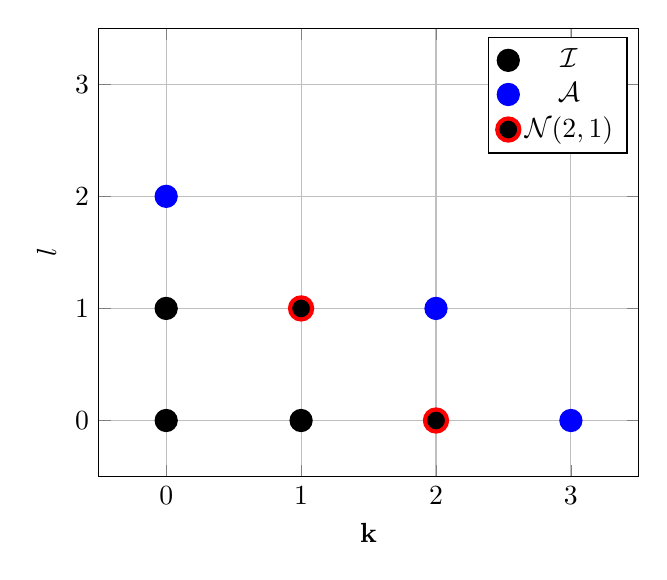
\begin{tikzpicture}

\begin{axis}[
xmin=-0.5, xmax=3.5,
ymin=-0.5, ymax=3.5,
axis on top,
xmajorgrids,
ymajorgrids,
xlabel=$\mi$,
ylabel=$l$
]
\addplot [only marks,mark size=4, draw=black, fill=black]
table {%
x                      y
+0.000000000000000e+00 +0.000000000000000e+00
+1.000000000000000e+00 +0.000000000000000e+00
+0.000000000000000e+00 +1.000000000000000e+00
+2.000000000000000e+00 +0.000000000000000e+00
+1.000000000000000e+00 +1.000000000000000e+00
};
\addplot [only marks, mark size=4,draw=blue, fill=blue]
table {%
x                      y
+3.000000000000000e+00 +0.000000000000000e+00
+2.000000000000000e+00 +1.000000000000000e+00
+0.000000000000000e+00 +2.000000000000000e+00
};
\addplot [only marks,mark size=4,line width=1.5, draw=red, fill=black]
table {%
x                      y
+1.000000000000000e+00 +1.000000000000000e+00
+2.000000000000000e+00 +0.000000000000000e+00
};
\addlegendentry{$\mis$};
\addlegendentry{$\mia$};
\addlegendentry{$\neighbors(2,1)$};
\end{axis}

\end{tikzpicture}
	\caption{Example with $d=1$ of a multi-index set $\mis$ and the associated set of admissible multi-indices $\mia$, as well as neighbors $\neighbors(2,1)$ of  $(2,1)\in\mia$. In this example $L=1$,  $\vsp_{1}=\vspan\{1,\psmi,\dots,\psmi^{6}\}=\vspan\{\leg_0(\psmi),\dots,\leg_{6}(\psmi)\}$, and  $\vsp_{0}=\vspan\{1,\psmi,\psmi^2\}=\vspan\{\leg_0(\psmi),\leg_1(\psmi),\leg_2(\psmi)\}$.}
	\label{fig:dc}
\end{figure}

We next explain how we arrive at the gain and work estimates that are required in step (i).
To estimate the norm of the orthogonal projection of $\rs_l-\rs_{l-1}$ onto $\pss_{\mi}$, we compute the arithmetic average of corresponding estimates for the neighbors $\neighbors(\mi,l)=\{(\mi^{(1)},l^{(1)}),\dots\}$ of $(\mi,l)$ in $\mathcal{I}$. Here, by neighbor we mean elements of $\mis$ that differ from $(\mi,l)$ in a single entry by $1$, see \Cref{fig:dc}.
For each such neighbor, we estimate the norm of the orthogonal projection $\operatorname{Proj}_{\mi^{(j)}}(\rs_{l^{(j)}}-\rs_{l^{(j)}-1})$ of $\rs_{l^{(j)}}-\rs_{l^{(j)}-1}$ onto $\pss_{\mi^{(j)}}$ simply by computing the Euclidean norm of those basis coefficients of $\P_{L-l^{(j)}}(\rs_{l^{(j)}}-\rs_{l^{(j)}-1})$ that belong to $\pss_{\mi^{(j)}}$. (Recall that $\P_{L-l^{(j)}}$ is a discrete projection onto the space $\vsp_{L-l^{(j)}}$ of which $\pss_{\mi^{(j)}}$ is a subspace since $\mi^{(j)}\in\mis_{l^{(j)}}$.)
The final estimate can be expressed as
\begin{equation*}
\frac{1}{|\neighbors(\mi,l)|}\sum_{j=1}^{|\neighbors(\mi,l)|}\norm{\operatorname{Proj}_{\mi^{(j)}}\P_{L-l^{(j)}}(\rs_{l^{(j)}}-\rs_{l^{(j)}-1})}{L^2_{\lambda}([0,1]^d)}.
\end{equation*}


To estimate the work that adding $(\mi,l)$ to $\mis$ incurs, we observe that \Cref{eq:adaptivestability} tells us exactly how many new samples are needed. More specifically, if we denote by $\NS(\mis_{l})$ the minimal solution of \Cref{eq:adaptivestability} for the polynomial subspace determined by $\mis_l$, then the required number of new samples of $\rs_{l}-\rs_{l-1}$ is $\NS(\mis_{l}\cup\{\mi\})-\NS(\mis_{l})$. It therefore remains to determine the  work per sample,  $\work(\rs_{l}-\rs_{l-1})$. If this work is unknown, then we store for each level $l$ an estimate, which we update with the observed computational work divided by the number of generated samples each time $\mathcal{I}_{l}$ changes. The final estimate of the work associated with $(\mi,l)$ is
\begin{equation*}
  \work(\rs_{l}-\rs_{l-1}) \cdot\left(\NS(\mis_{l}\cup\{\mi\})-\NS(\mis_{l})\right).
\end{equation*}

%\Cref{fig:dc} shows an example of $\mis$ and $\mia$ in the case $d=1$. In this case, the polynomial subspaces are simply spaces of polynomials with degree less than or equal to some natural number; more specifically, \Cref{fig:dc} represents the case
\Cref{alg:adaptive} gives a summary of our algorithm in pseudocode.
%\begin{rem}[Alternative multilevel construction]
%From the description of the multilevel method in terms of multi-indices as in \Cref{fig:dc}, one sees that one could alternatively first group all the indices that agree in the $\mi$ component instead of the $l$ component, which would yield approximations of the form
%$$
%\P_{\vsp_{0}}f_{L}+\sum_{l=1}^{L}\P_{\vsp_l\ominus \vsp_{l-1}}\rs_{L-l},
%$$
%where $\vsp_{l}\ominus\vsp_{l-1}$ denotes the orthogonal complement of $\vsp_{l-1}$ %in $\vsp_{l}$.
%\end{rem}


\begin{algorithm}[ht]
\caption{Adaptive multilevel algorithm.}\label{alg:adaptive}
\begin{algorithmic}[1]
		\Function{MLA}{$(\rs_l)_{l\in\N}$,STEPS}
		\State  $\mis\gets \{\mathbf{0}\}$
		\State $X_l\gets \varnothing\;\forall l\in\N$
		\State $\Delta_l\gets 0\;\forall l\in\N$
		\For{$0\leq i<\text{STEPS}$}
			\State $(\mi,l)\gets \argmax_{(\mi,l)\in\mia}\frac{\text{GAIN}((\mi,l),(\Delta_l)_{l\in\N},\mis)}{\text{WORK}((\mi,l),\mis)}$
			\State $N_{+}\gets \NS(\mis_{l}\cup\{\mathbf{k}\})-\NS(\mis_{l})$
			\State $\mis\gets \mathcal{I}\cup\{(\mi,l)\}$
			\For{$0\leq j<N_{+}$}
				\State Generate $\psmi\sim \arcsine_{d}$
				\State $y\gets (\rs_{l}-\rs_{l-1})(\psmi)$
				\State $X_l\gets X_l\cup\{(\psmi,y)\}$
			\EndFor
			\State $\Delta_l\gets \P_{L-l}(\rs_{l}-\rs_{l-1})$
		\EndFor
		\State \Return $\sum_{0\leq l\leq L}\Delta_l$
	\EndFunction
	\item[]
	\Function{GAIN}{$(\mi,l)$,$(\Delta_l)_{l\in\N}$,$\mathcal{I}$}
		\State $s=0$
		\For{$(\mi^{(j)},l^{(j)})\in \neighbors(\mi,l)$}
			\State $s\gets s+\|\operatorname{Proj}_{\mi^{(j)}}\Delta_{l^{(j)}} \|_{L^2_{\lambda}}$
		\EndFor

		\State \Return $s/|\neighbors(\mathbf{k},l)|$
	\EndFunction
	\item[]
	\Function{WORK}{$(\mi,l)$,$\mathcal{I}$}
		\State \Return $\work(\rs_{l}-\rs_{l-1})\cdot\left(\NS(\mis_{l}\cup\{\mi\})-\NS(\mis_{l})\right)$
	\EndFunction

\end{algorithmic}
\end{algorithm}

\section{Application to parametric PDE}
\label{sec:uq}
%In this section, we discuss the applicability of \Cref{thm:main,thm:main2} to problems in uncertainty quantification.

We assume in this section that $\pde(\cdot,\psmi)$ is the solution of some partial differential equation (PDE) with parameters $\psmi\in\domPS\subset\R^\dps$ and that we are interested in the \emph{response surface}
\begin{equation*}
\psmi\mapsto \rs_{\infty}(\psmi):=\QoI(\pde(\cdot,\psmi))\in\R,
\end{equation*}
where $\QoI(\pde(\cdot,\psmi))$ is a real-valued quantity of interest, such as a point evaluation, a spatial average, or a maximum.  
In most situations, we cannot evaluate $\rs_{\infty}(\psmi)$ exactly, as this would require an analytic solution of the PDE. Instead, we have to work with discretized solutions $\pde_{n}(\cdot,\psmi)$ for each $\psmi$, which yield approximate response surfaces
\begin{equation*}
\begin{split}
\rs_{n}\colon &\domPS\to\R \\
&\psmi\mapsto Q(\pde_{n}(\cdot,\psmi)).
\end{split}
\end{equation*}
For example, if we employ finite element discretizations with maximal element diameter $h:=n^{-1}$, then the work required for evaluations of $\rs_{n}$ grows like $h^{-\gamma}=n^{\gamma}$ for some $\gamma>0$. To apply the multilevel method of \Cref{sec:nonadaptive}, we need to verify the remaining Assumptions A1 and A2 from there. 

%consider parametric partial differential equations of the form
%\begin{equation}
%\label{eq:PDE}
%\begin{split}
%\PDE_y(u)=\rs_y
%\end{split}
%\end{equation}
%where both operator  $\PDE_y$ and right-hand side $\rs_y$ may depend on a %parameter $y\in\domPS\subset\mathbb{R}^d$ with $d\in\N\cup\{\infty\}$.%
% Assuming that there is a unique solution $u_y:=\PDE_y^{-1}(\rs_y)$ for each $y\in\domPS$, our goal is to approximate the dependence of a scalar, possibly nonlinear, quantity of interest $\qoi(u_y)$ on the parameter $y$.
As a motivating example, we consider a linear elliptic second order PDE, which has been extensively studied in recent years \cite{harbrecht2013multilevel,ChkifaCohenSchwab2015,CohenDevoreSchwab2011,BabuskaTemponeZouraris2004},
\begin{equation}
\label{eq:UQex}
\begin{aligned}
-\nabla \cdot (a(x,\psmi) \nabla \pde(x,\psmi))&=\rhs(x)&\text{ in }U\subset\R^{\dpde}\\
\pde(x,\psmi)&=0&\text{ on } \partial U,
\end{aligned}
\end{equation}
with $a:U\times \domPS\to\R$ and $\domPS:=[0,1]^\dps$. 


%If $\rhs\in H^{-1}(U)$ and
%\begin{equation}
%\inf_{x\in U}a(x,\psmi)>0\quad \forall \psmi\in\domPS,
%\end{equation}
%then the Lax-Milgram theorem guarantees existence of a unique solution $\pde(\cdot,\psmi)\in H_0^1(U)$ for all $\psmi\in\domPS$. In order to obtain convergence of 
\begin{pro}
	\label{pro:finite}
	For any $n\in\N$, let $\pde_{n}$ be finite element approximations of order $r\geq 1$ and maximal element diameter $h:=(n+1)^{-1}$, and let $\rs_{n}(\psmi):=Q(\pde_n(\cdot,\psmi))$.
	Assume that $g$ and $U$ are sufficiently smooth, that 
	\begin{equation}
		\inf_{x\in U,\psmi\in\domPS}a(x,\psmi)>0,
	\end{equation}
	and that $Q$ is a continuous linear functional on $L^2(U)$.
	
	
	
	\begin{enumerate}[(i)]
		\item If $a\in C^{r}(U\times\domPS)$ for some $r\geq 1$, then  %$\norm{\partial_{x}^{\mathbf{r}}\partial_{\psmi}^{\mathbf{s}}a}{C^0(U\times \domPS)}<\infty$ for all $|\mathbf{r}|_{1}+|\mathbf{s}|_{1}\leq r$, then 
		\begin{equation*}
		\norm{\rs_{\infty}-\rs_{n}}{L^2(\domPS)}\lesssim h^{r+1}
		\end{equation*}
		and
		\begin{equation*}
		\norm{\rs_{\infty}-\rs_{n}}{C^{r-1}(\domPS)}\lesssim h^{2}.
		\end{equation*}
		\item If for some $r,s\geq 1$ we have
		\begin{equation}
		\label{eq:tensor}
		\begin{split}
		a\in C^{r}(U)\otimes C^{s}(\domPS):=\{a\colon U\times \domPS\to\R :  \norm{\partial_{x}^{\mathbf{r}}\partial_{\psmi}^{\mathbf{s}}a}{C^0(U\times\domPS)}<\infty\;\forall\;|\mathbf{r}|_{1}\leq r,|\mathbf{s}|_{1}\leq s\}
		,
		\end{split}
		\end{equation} then 
		\begin{equation*}
		\norm{\rs_{\infty}-\rs_{n}}{C^{s}(\domPS)}\lesssim h^{r+1}.
		\end{equation*}
		
	%	\item If there exists $s\geq $ such that $\norm{\partial_{x}^{\mu}\partial_{\psmi}^{\nu}a}{C^0(U\times \domPS)}<\infty$ for all $|\mu|_{1}\leq r,|\nu|_{1}\leq s$ for some $s\geq 1$, then 
	%	\begin{equation*}
	%	\norm{\rs_{\infty}-\rs_{n}}{C^{s}_{\mix}(\domPS)}\lesssim h^{r+1}.
	%	\end{equation*}
	\end{enumerate}
\end{pro}
\begin{proof}
	In both cases, the standard theory of second order elliptic differential equations shows that $\psmi\mapsto \pde(\cdot,\psmi)$ is well defined as a map from $\domPS$ into $H^{r+1}(U)$, with 
	\begin{equation*}
	\norm{\pde}{L^\infty(\domPS;H^{r+1}(U))}<\infty.
	\end{equation*}
	Next, we observe that the derivatives $\partial_{\psmi_{j}}\pde(\cdot,\psmi)$, $j\in \{1,\dots,d\}$ satisfy PDEs with the same operator as in \Cref{eq:UQex} but with new right-hand sides
	\begin{equation*}
	\tilde{\rhs}(x):=\nabla\cdot(\partial_{\psmi_j}a(x,\psmi)\nabla \pde(x,\psmi)).
	\end{equation*}
	The regularity of this right-hand side now depends on the assumptions on the coefficient $a$.
	In case (i) we have $\partial_{\psmi_j}a(\cdot,\psmi)\in C^{r-1}(U)$ and thus $\tilde{\rhs}\in H^{r-2}(U)$. Therefore, $\partial_{\psmi_{j}}\pde(\cdot,\psmi)\in H^{r}(U)$ for each $\psmi\in\domPS$ and, moreover, we have the uniform estimate
		\begin{equation*}
		\norm{\partial_{\psmi_j}\pde}{L^\infty(\domPS;H^{r}(U))}<\infty.
		\end{equation*}
		In case (ii) we have $\partial_{\psmi_j}a(\cdot,\psmi)\in C^{r}(U)$ and thus $\tilde{\rhs}\in H^{r-1}(U)$. Therefore, $\partial_{\psmi_{j}}\pde(\cdot,\psmi)\in H^{r+1}(U)$ for each $\psmi\in\domPS$ and, moreover, we have the uniform estimate
		\begin{equation*}
		\norm{\partial_{\psmi_j}\pde}{L^\infty(\domPS;H^{r+1}(U))}<\infty.
		\end{equation*}
		Repeatedly applying these arguments yields
			\begin{equation*}
			\norm{\pde}{C^{r-1}(\domPS;H^2(U))}<\infty,
			\end{equation*}
			and
			\begin{equation*}
			\norm{\pde}{C^{s}(\domPS;H^{r+1}(U))}<\infty,
			\end{equation*}
%			or
%			\begin{equation*}
%			\norm{\pde}{C^{s}_{\mix}(\domPS;H^{r+1}(U))}<\infty,
%			\end{equation*}
		in cases (i) and (ii), respectively. We may now conclude by using standard finite-element theory. In case (i), we have
		\begin{equation*}
		\begin{split}
		\norm{\rs_{\infty}-\rs_{n}}{L^2(\domPS)}&\leq \norm{Q}{}\norm{\pde-\pde_{n}}{L^2(\domPS;L^2(U))}\\
		&\lesssim h^{r+1}\norm{\pde}{L^2(\domPS;H^{r+1}(U))}
		\end{split}
		\end{equation*}
		and
		\begin{equation*}
		\begin{split}
		\norm{\rs_{\infty}-\rs_{n}}{C^{r-1}(\domPS)}&\lesssim \norm{\pde-\pde_{n}}{C^{r-1}(\domPS;L^2(U))}\\
		&\lesssim h^{2}\norm{\pde}{C^{r-1}(\domPS;H^{2}(U))},
		\end{split}
		\end{equation*} 
	whereas in case (ii), we have
	\begin{equation*}
	\begin{split}
	\norm{\rs_{\infty}-\rs_{n}}{C^{s}(\domPS)}&\lesssim \norm{\pde-\pde_{n}}{C^{s}(\domPS;L^2(U))}\\
	&\lesssim h^{r+1}\norm{\pde}{C^{s}(\domPS;H^{r+1}(U))},
	\end{split}
	\end{equation*}
\end{proof}
\begin{rem}
In case (i) of the previous proposition, differentiating with respect to $\psmi$ reduces the number of available derivatives in $x$, which are required for convergence of the finite element method. Thus, the convergence in $L^2(\domPS)$ is faster than that in $C^{r-1}(\domPS)$. Case (ii), on the other hand, describes the so-called \emph{mixed smoothness} of the coefficient in $x$ and $\psmi$, meaning that differentiating in $\psmi$ does not affect the differentiability with respect to $x$.  
\end{rem}
 % Roughly speaking, it can be shown that for \Cref{eq:UQex} the response surface $\rs_{\infty}$ is as regular with respect to $\psmi$ as the diffusion coefficient $a_{\psmi}$. For example, if $a_{\psmi}$ is $s$ times differentiable with respect to $\psmi$ and the functional $\QoI$ is $s$ times differentiable with respect to $u$ (both in a suitable sense), then $\rs_{\infty}$ is $s$ times differentiable as well. % and lies in a Sobolev or a Hölder space of functions on $\domPS$ depending on the specifics of the problem and on the integrability of the derivatives $\partial^{s}_{\psmi}a_{\psmi}$. 
If the coefficients depend analytically on $\psmi$, then the same holds for $\rs_{\infty}$, which can be exploited to obtain algebraic polynomial approximability rates of $\rs_{\infty}$ even in the case of infinite-dimensional parameters \cite{ChkifaCohenSchwab2015,Haji-AliNobileTamelliniEtAl2015}, as shown below.

%However, to obtain strong convergence, we need not only know that $\rs_{\infty}\in \F$  for some space $\F$ with good polynomial approximability properties, but that 
%\begin{equation*}
%\norm{\rs_{\infty}-\rs_{n}}{\F}\lesssim n^{-\sc}
%\end{equation*}
%for some $\sc>0$. Estimates of this type have been established for example in \cite{harbrecht2013multilevel,Haji-AliNobileTamelliniEtAl2015}. An example of such an estimate is provided in \Cref{pro:UQ} below. 

%The underlying idea of this example is that the strong convergence rate $\sc=1$ can usually be obtained in any space $\F$ such that $\rs_{\infty}\in \F$. 

\begin{pro}
\label{pro:UQ}
Let $\domPS:=[-1,1]^{\infty}$.
Assume that $Q$ is a linear and continuous functional on $L^2(U)$, that $0<\inf_{x,\psmi}  a(x,\psmi)\leq \sup_{x,\psmi}  a(x,\psmi)<\infty$, and that
	\begin{align*}
	a(x,\psmi)&=\bar{a}(x)+\sum_{j=0}^{\infty}\ps_j\psi_j(x),\\
		a(x,\psmi)&=\bar{a}(x)+\left(\sum_{j=0}^{\infty}\ps_j\psi_j(x)\right)^2,\quad \\
	\intertext{or}
		a(x,\psmi)&=\exp\left(\sum_{j=0}^{\infty}\ps_j\psi_j(x)\right). 
	\end{align*}
	If there exists $r_{\max}>1$ such that
	\begin{equation*}
	 \|\psi_j\|_{C^{r}(U)}\lesssim (j+1)^{-(r_{\max}+1 - r)}\quad\forall j\in\N, \; 0\leq r< r_{\max},
	 \end{equation*} 
	 	 then, for any $r\in \N$ with $1\leq r< r_{\max}$, finite element approximations with maximal element diameter $h:=(n+1)^{-1}$ achieve
\begin{equation*}
\norm{\rs_{\infty}-\rs_{\n}}{L^{\infty}(\domPS)}\leq C h^{r+1}
\end{equation*}
with a constant $C$ independent of $n$.
Furthermore, for any such $r$, there is a sequence $(\vsp_\dvsp)_{\dvsp\in\N}$ of downward closed polynomial spaces with $\dim \vsp_\dvsp=m$ such that finite element approximations with order $r$ and maximal diameter $h:=(n+1)^{-1}$ achieve 
\begin{equation*}
e_{\vsp_\dvsp,1,\infty}(\rs_{\infty}-\rs_\n)\leq C(\dvsp+1)^{-\uqsummability}h^{r+1} \quad \forall\, 0<\uqsummability<r_{\max}- r
\end{equation*}
with a constant $C$ independent of $n$ and $m$.
%and
%\begin{equation*}
%e_{\vsp_\dvsp,2}(\rs_{\infty}-\rs_\n)\leq C(\dvsp+1)^{-\uqsummability}h^{r+1},\quad \forall \uqsummability<r_{\max}-\delta r-\frac{1}{2}
%\end{equation*}
\end{pro}
\begin{proof}
	
	It was shown in \cite[Theorem 4.1 \& Section 5]{ChkifaCohenSchwab2015} that for each $0\leq r<r_{\max}$ there exists a set $\domPS_{r}\subset \C^{\infty}$, $\domPS\subset \domPS_{r}$ such that
	$\norm{a}{L^{\infty}(\domPS_{r};C^{r}(U))}<\infty$ and such that $\psmi\mapsto \pde(\cdot,\psmi)$ may be extended to a complex differentiable map from $\domPS_{r}$ into $H^{1+r}(U)$ with
		\begin{equation}
		\label{eq:complexbounds}
		\begin{split}
	\norm{\pde}{L^{\infty}(\domPS_{r};H^{1+r}(U))}<\infty
		\end{split}
		\end{equation}
	
For a detailed description of the sets $\domPS_{r}$ we refer to \cite{ChkifaCohenSchwab2015}. For our purposes it suffices to know that the better the summability of $(\norm{\psi_j}{C^{r}(U)})_{j\in\N}$, the larger $\domPS_{r}$ can be chosen; and the larger $\domPS_{r}$ the better the polynomial approximability properties of complex differentiable maps defined on $\domPS_{r}$.
In particular, the results of \cite[Section 2]{ChkifaCohenSchwab2015}, show that when  restricted to the smaller set $\domPS$ such maps may be approximated at algebraic convergence rates within downward closed polynomial subspaces. More specifically, \cite[Equation (2.27)]{ChkifaCohenSchwab2015} shows that if a function $e$ is complex differentiable on $\domPS_{r}$, then for any $\dvsp\in\N$ there exists a downward closed polynomial subspace $\vsp_{\dvsp}$ such that
	\begin{equation*}
	\begin{split}
	\inf_{\tilde{\p}\in \vsp_{\dvsp}\otimes L^2(U)}\norm{e-\tilde{\p}}{L^\infty(\domPS;L^2(U))}\lesssim (\dvsp+1)^{-\alpha} \norm{e}{L^\infty(\domPS_{r};L^2(U))}
	\end{split}
	\end{equation*}
	for all $\alpha<r_{\max}- r$. 
 Applying this estimate with $e:=\pde-\pde_{n}$ shows
	\begin{equation*}
	\begin{split}
	\inf_{\p\in\vsp_{\dvsp}}\norm{(\rs_{\infty}-\rs_{\n})-\p}{L^\infty(\domPS)}&\leq \norm{Q}{} \inf_{\tilde{\p}\in \vsp_{\dvsp}\otimes L^2(U)}\norm{(\pde-\pde_n)-\tilde{\p}}{L^\infty(\domPS;L^2(U))}\\
\lesssim & (\dvsp+1)^{-\alpha} \norm{\pde-\pde_{n}}{L^\infty(\domPS_{r};L^2(U))}.
	\end{split}
	\end{equation*}

By standard finite element analysis we finally obtain
\begin{equation*}
\norm{\pde-\pde_{n}}{L^{\infty}(\domPS_{r};L^2(U))}\leq C h^{r+1}\norm{\pde}{L^{\infty}(\domPS_{r};H^{r+1}(U))}.
\end{equation*}
with  $C=C\big(	\norm{a}{L^{\infty}(\domPS_{r};C^{r}(U))}\big)<\infty$. Combining the previous two estimates with \Cref{eq:complexbounds} concludes the proof.
\end{proof}

\begin{rem}
	Similar results can also be shown for PDEs of parabolic type and for some nonlinear PDEs \cite{ChkifaCohenSchwab2015}.
\end{rem}
% !TEX root = main.tex

\begin{figure*}[t!]
  \centering
\includegraphics[width=0.325\textwidth]{./figs/0_simp_c1c2.pdf}
\includegraphics[width=0.315\textwidth]{./figs/0_simp_c3c4.pdf}
\includegraphics[width=0.26\textwidth]{./figs/0_simp_quad_bnds.pdf}
  \caption{We verify that the performative risk bounds in Assumption~\ref{ass:exist_V} are satisfied in the example discussed in Section~\ref{sec:example}. (a) As a function of $r$ (the radius of the domain where the inequalities hold), we show the tightest constants $c_1$ and $c_2$ for the bound. We also plot $\sqrt{c_1/c_2}r$, which is the radius of a neighborhood of $x=0$ to which Theorem~\ref{th:perturb1} can be applied. (b) As a function of $r$, we show the tightest constants for $c_3$ and $c_4$. (c) Choosing the $c_1$ and $c_2$ constants for $r = 0.5$, we visualize how the quadratic bounds hold for the performative risk locally.}
  \label{fig:simp_ex_demo}
\end{figure*}
In this section, we revisit the models introduced in Section~\ref{sec:example}. We demonstrate how the results of Sections~\ref{sec:analysis_prm} and~\ref{sec:analysis_RGD} can be applied. First, we show that the example satisfies Assumption~\ref{ass:exist_V} and we calculate its corresponding constants. Second, we apply Theorem~\ref{th:perturb1} and show the theoretical convergence rates match simulated trajectories. 
Finally, we also apply Theorem~\ref{th:perf_align} to the example from Section~\ref{sec:simple_ex} and characterize the class of distribution shifts satisfy the performative alignment condition.

\subsection{Checking the curvature of the performative risk and region of convergence}

Recall the example from Section~\ref{sec:simple_ex}, where $x$ was a scalar, the loss function was the squared error, and the decision-dependent distribution was a Bernoulli random variable whose distribution was determined by $p(\cdot)$. In this section, we consider the specific decision-dependent distribution shift $p = \varphi$, which is defined in Equation~\eqref{eq:varphi_def}.

When we consider this example, we can see that the bounds on Assumption~\ref{ass:exist_V} cannot hold globally, which matches our previous observation that there are multiple isolated performative risk minimizers. However, these bounds may hold locally: we can view the constants $(c_i)_{i=1}^4$ from Assumption~\ref{ass:exist_V} as a function of the size of the domain $r$.

For concreteness, let us focus on the equilibrium point $x = 0$. Recall that Assumption~\ref{ass:exist_V} must hold locally, on the domain $\{ x : |x-x^*| \le r\}$. As we increase $r$, the constants will worsen; we visualize this in Figure~\ref{fig:simp_ex_demo}(a)--(b). Note that these bounds only have to hold locally around the equilibria, as visualized in Figure~\ref{fig:simp_ex_demo}(c). Furthermore, the gradient bounds in Assumption~\ref{ass:exist_V} cannot hold beyond $r > 0.40$, since $\nabla PR(x) = 0$ at that point.

Recall that the convergence results of Theorem~\ref{th:perturb1} can only apply to all initial conditions satisfying $|x_0 - x^*| < \sqrt{c_1/c_2}r$; we visualize this as well in Figure~\ref{fig:simp_ex_demo}(a). 
On the set $(0,0.40]$, we can see the quantity $\sqrt{c_1/c_2}r$ is the largest at $r = 0.4$, with constants $c_1 = 0.50$ and $c_2 = 1.78$. 
Thus, around the equilibrium $x = 0$, the theorem can be applied to all points in the set $\{ x : |x| \le 0.21 \}$, with $\delta = 0$. Thus, our theorem shows that all points in this neighborhood of $x = 0$ will converge. This under-approximates the true region of attraction, which we numerically saw to be $\{ x : x < 0.23 \}$.



\subsection{Performative alignment with squared error and Bernoulli distributions}
\label{sec:perf_align_ex}

We again consider the example from Section~\ref{sec:simple_ex}. However, in this section, we consider a general decision-dependent distribution shift $p(\cdot)$. 
% Recall the example from Section~\ref{sec:simple_ex}, where $x$ was a scalar, the loss function was the squared error, and the decision-dependent distribution was a Bernoulli random variable whose distribution was determined by $p(\cdot)$.  
We suppose that $p(0) = 0$ and $p(1) = 1$, so we have two performative risk minimizers as in our previous example. We have $\nabla_{x_1}R(x,x) = x - p(x)$ and $\nabla_{x_2}R(x,x) = (1/2 - x) p'(x)$. 
The performative alignment condition becomes:
\begin{equation}
    \label{eq:perf_align_ex}
    |1/2 - x|^2 |p'(x)|^2 \le (p(x)-x)(1/2 - x)p'(x)
\end{equation}
Theorem~\ref{th:perf_align} states that if this condition holds for all $x \in (0,c)$, then any initial conditions $x_0 \in (0,c)$ will converge to $x = 0$. Similarly, if this condition holds for all $x \in (c,1)$, then all initial conditions in $(c,1)$ will converge to $x = 1$. Theorem~\ref{th:perf_align} also implies that this condition cannot be satisfied for all $x \in (0,1)$, as then these initial conditions would converge to \textit{both} $x = 0$ and $x = 1$.

If we suppose that $p(\cdot)$ is monotonic on $(0,1)$, i.e. $p'(x) \ge 0$, we can also interpret the performative alignment condition as follows. For $x \in (1/2,1)$, the performative alignment condition becomes $p(x) - x \ge (1/2 - x)p'(x)$. In this regime, $(1/2 - x)p'(x) \le 0$. In this setting, if $p(x) - x$ is too negative, the RGD flow will push $x$ away from the nearby minimizer $x = 1$. Similarly, for $x \in (0,1/2)$, the condition becomes $p(x) - x \le (1/2 - x)p'(x)$. In this regime, $(1/2 - x)p'(x) \ge 0$, and the condition states that $p(x) - x$ cannot be too large, or the RGD flow will push $x$ away from the minimizer $x = 0$.

In this section, we used Theorem~\ref{th:perf_align} to identify conditions on the decision-dependent distribution shift $p(\cdot)$ which ensure that the performative risk does not increase even when the dynamics follow repeated gradient descent.
For this example, the condition is that $p$ satisfies Equation~\eqref{eq:perf_align_ex} for all $x \in (0,c)$. 
More generally, the performative alignment condition allow us to specify a class of distribution shifts which behave well with respect to performative risk minimization.



\begin{comment}
\begin{figure}
\includegraphics[width=\linewidth]{figs/beyond_tss_lesion.pdf}
\caption[]{End-to-End runtime lesion study of the entire MNIST dataset and the FMA featurized music dataset. Each of DROP's contributions provides a runtime improvement.}
\label{fig:beyond_lesion}
\end{figure}
\end{comment}



\section{Conclusion}
\label{sec:conclusion}

Advanced data analytics techniques must scale to rising data volumes. 
DR techniques offer a powerful toolkit when processing these datasets, with PCA frequently outperforming popular techniques in exchange for high computational cost. 
In response, we propose DROP, a new dimensionality reduction optimizer. 
DROP combines progressive sampling, progress estimation, and online aggregation to identify high quality low dimensional bases via PCA without processing the entire dataset by balancing the runtime of downstream tasks and achieved dimensionality. 
Thus, DROP provides a first step in bridging the gap between quality and efficiency in end-to-end DR for downstream \red{analytics}. 

%We revisit canonical operators for time series dimensionality reduction and the measurement study of~\cite{keogh-study}, and show that PCA is more effective than popular alternatives in the data mining literature often by a margin of over $2\times$ on average on gold-standard time series benchmark data sets with respect to output data dimension. More surprisingly, we empirically demonstrate that a small number of samples are sufficient to accurately characterize directions of maximum variance and obtain a high-quality low-dimensional transformation.



\paragraph{Acknowledgements} F. Nobile received support from the Center for ADvanced MOdeling Science (CADMOS). R. Tempone and S. Wolfers are members of the KAUST SRI Center for Uncertainty Quantification in Computational Science and Engineering. R. Tempone received support from the KAUST CRG3 Award Ref:2281 and the KAUST CRG4 Award Ref:2584.



%\clearpage
%\listoffigures
%\addcontentsline{toc}{section}{\refname}\printbibliography

\bibliography{library.bib}{}
\bibliographystyle{plain}
\end{document}
